\documentclass[a4paper,12pt,oneside]{book}
\usepackage[utf8]{inputenc}
\usepackage{amssymb}
\usepackage{amsmath}
\usepackage{graphicx}
\graphicspath{ {images/} }
\usepackage{times}
\usepackage{geometry}
\usepackage{setspace}
\usepackage{tocloft}
\usepackage{tabu}
\usepackage{fancyhdr}
\geometry{a4paper, tmargin=1in, rmargin=1in, bmargin=1in, lmargin=1.5in}


%-----------------------------------------
% Editables of the document
%-----------------------------------------
\newcommand{\thesistitle}{SKILL-GAP \& CURRICULUM DRIFT INTELLIGENCE FOR UNIVERSITIES} % Title of the Thesis, change here
\newcommand{\shorttitle}{SKILL-GAP \& CURRICULUM DRIFT INTELLIGENCE FOR UNIVERSITIES} % running header
\newcommand{\thesisauthora}{Siri Jeendru (160124771021)} % Person 1
\newcommand{\thesisauthorb}{Anugnya Somishetty (160124771023)} % Person 2
\newcommand{\thesisauthorc}{Murari Geddam (160124771039)} % Person 3
% If the number of people is different, change accordingly in titlepage and bonafide -certificate
\newcommand{\thesisdept}{Artificial Intelligence and Data Science} % Department
\newcommand{\thesisguide}{Dr. T. Satya Kiranmai} % Project Guide (as in the team's report MP_main_report.docx)
\newcommand{\thesisguidedesignation}{Assistant Professor} % as in the team's report; the updated template's sample title page says Associate Professor -- confirm
\newcommand{\depthod}{Prof. K. Radhika} % Department Head
% Also, change the graduation year in titlepage and bonafide certificate
%-----------------------------------------

% References are to be added in reference.bib and cited in any part of the document. Read any examples online on how to add references. You can also use Google Scholar to get the reference formatted for BibTex.


% For Figures and Subfigures
\usepackage{graphicx, caption, subcaption}

% Package for block commenting
\usepackage{comment}

\usepackage{physics}

% Package to keep images in place
\usepackage{float}

% Package for Appendices
\usepackage{titletoc}
\usepackage{appendix}

% Chapter and Appendix in TOC prefixed
\makeatletter
\titlecontents{chapter}%
 [0pt]% 
 {\bfseries}%
 {\MakeUppercase \@chapapp\ \thecontentslabel\quad}% 
 {}% 
 {\normalfont\cftdotfill{\cftdotsep}\contentspage}% 
 [\addvspace{0pt}]% 

\g@addto@macro\appendices{%
  \addtocontents{toc}{\protect\renewcommand{\protect\@chapapp}{\appendixname}}%
}
\makeatother


% Package for codes
\usepackage{listings}
\lstset{
    breaklines = true,
    captionpos = b,
    numberstyle = \scriptsize,
    numbers=left,                    
    numbersep=10pt
}


% Package for enumerate
\usepackage{enumitem}

% Block Diagram Packages and Functions
\usepackage{tikz}
\usetikzlibrary{arrows, decorations.markings}
\usetikzlibrary{arrows,positioning,shapes.geometric}
\tikzstyle{vecArrow} = [thick, decoration={markings,mark=at position
   1 with {\arrow[semithick]{open triangle 60}}},
   double distance=1.4pt, shorten >= 5.5pt,
   preaction = {decorate},
   postaction = {draw,line width=1.4pt, white,shorten >= 4.5pt}]
\tikzstyle{innerWhite} = [semithick, white,line width=1.4pt, shorten >= 4.5pt]
\tikzstyle{block} = [draw, fill=blue!20, rectangle, 
    minimum height=3em, minimum width=6em]

% Chapter Title Customization
\usepackage{titlesec}
%\titleformat{\chapter}[display]% OLD
%    {\normalfont\huge\bfseries}{\chaptertitlename\ \thechapter}{20pt}{\Huge}% OLD
% \titlespacing*{\chapter}{0pt}{50pt}{40pt}% OLD

\titleformat{\chapter}[display]
{\Large\bfseries\centering}{\MakeUppercase\chaptertitlename\ \thechapter}{5pt}{\Large}
\titlespacing*{\chapter}{0pt}{0pt}{20pt}

% Section Customization
\titleformat{\section}{\large \bfseries}{\thesection}{1em}{}

% Sub-Section Customization
\titleformat{\subsection}{\fontsize{13pt}{13pt} \bfseries}{\thesubsection}{1em}{}


% Align the titles of auxiliary content to center
\renewcommand*\contentsname{\Large \centerline{TABLE OF CONTENTS}}
\renewcommand*\listfigurename{\Large \centerline{LIST OF FIGURES}}
\renewcommand*\listtablename{\Large \centerline{LIST OF TABLES}}


% Tables, colours and plots used by the report (added; not in the original template)
\usepackage{booktabs}
\usepackage{longtable}
\usepackage{tabularx}
\usepackage{multirow}
\usepackage[table]{xcolor}
\usepackage{pgfplots}
\pgfplotsset{compat=1.18}
\usetikzlibrary{fit,calc,backgrounds}
\usepackage{amsthm}
\lstdefinestyle{repo}{language=Python, basicstyle=\ttfamily\scriptsize, keywordstyle=\bfseries, commentstyle=\itshape\color{gray!70!black}, stringstyle=\color{black!80}, numbers=left, numberstyle=\tiny\color{gray}, numbersep=6pt, frame=single, rulecolor=\color{gray!60}, backgroundcolor=\color{gray!6}, breaklines=true, breakatwhitespace=false, postbreak=\mbox{\textcolor{gray}{$\hookrightarrow$}\space}, columns=fullflexible, keepspaces=true, showstringspaces=false, xleftmargin=1.6em, framexleftmargin=1.4em, upquote=true} % added: code attachments
\setlength{\LTcapwidth}{\textwidth}
\setlength{\emergencystretch}{2.5em} % added: lets lines with long file paths break
% Relationship labels of the project's schema (relationship-labels-v1), typeset consistently
\DeclareRobustCommand{\lbl}[1]{\begingroup\def\_{\textunderscore\allowbreak}\textsf{\small #1}\endgroup}
\newcommand{\SC}{\lbl{SAME\_CONCEPT}}
\newcommand{\PA}{\lbl{PARENT}}
\newcommand{\CH}{\lbl{CHILD}}
\newcommand{\RE}{\lbl{RELATED}}
\newcommand{\PO}{\lbl{PARTIAL\_OVERLAP}}
\newcommand{\UN}{\lbl{UNRELATED}}
\newcommand{\AM}{\lbl{AMBIGUOUS}}
\newcommand{\IE}{\lbl{INSUFFICIENT\_EVIDENCE}}
\DeclareRobustCommand{\code}[1]{\begingroup\def\_{\textunderscore\allowbreak}\texttt{\small #1}\endgroup}
% table rows generated from the recomputed results; primitive input so rows can sit inside tabular/longtable
\makeatletter\newcommand{\inputrows}[1]{\@@input #1 }\makeatother

% References Addition
\usepackage[backend=bibtex,
style=numeric,
bibencoding=ascii,
maxbibnames=99,
sorting=none
%style=alphabetic
%style=reading
]{biblatex}
\addbibresource{reference.bib}

% Page Style
\setlength{\headheight}{15pt} % added: fancyhdr needs at least 14.5pt
\pagestyle{fancy}
\cfoot{\thepage}
\rhead{}
\lhead{}
\renewcommand{\headrulewidth}{0pt}
\renewcommand{\footrulewidth}{0pt}

% Line Spacing
\usepackage{setspace}

% Indent First Paragraph
\usepackage{indentfirst}

% To make uppercase words
\usepackage{textcase}


\usepackage[bookmarks, colorlinks=false, pdfborder={0 0 0}, pdftitle={\thesistitle}, pdfkeywords={}]{hyperref}


\begin{document}

% To expand the word spacing
\spaceskip=1.5\fontdimen2\font plus 1.5\fontdimen3\font
minus 1.5\fontdimen4\font


\frontmatter
\pagenumbering{gobble}
\begin{titlepage}
\begin{center}
\fontsize{20pt}{1cm}\selectfont \textbf{\thesistitle}

\vspace*{0.8cm}
\fontsize{14pt}{21pt}\selectfont A Mini Project Report \\
submitted in partial fulfillment of the requirements for \\
the award of the degree of

\vspace*{0.3cm}
\fontsize{14pt}{1cm}\selectfont\textbf{Bachelor of Engineering} 

\vspace*{0.3cm}
\textbf{in\\\thesisdept}

\vspace*{0.5cm}
By

\textbf{\thesisauthora}\\
\textbf{\thesisauthorb}\\
\textbf{\thesisauthorc}\\
\vspace*{0.5cm}
\textbf{\textit{Under the esteemed guidance of}}\\
\textbf{\thesisguide}\\
\thesisguidedesignation\\
\vfill

\includegraphics[width=1.25in]{cbit.png}

\vspace*{0.3in}
\fontsize{12pt}{12pt}\selectfont \textbf{DEPARTMENT OF ARTIFICIAL INTELLIGENCE AND DATA SCIENCE}\\[0.2cm]
\fontsize{14pt}{14pt}\selectfont\textbf{CHAITANYA BHARATHI INSTITUTE OF TECHNOLOGY}\\[0.2cm]
\textbf{HYDERABAD -- 500075}

\vspace*{0.2cm}
\textbf{NOVEMBER 2026}
\end{center}
\end{titlepage}
\thispagestyle{empty}
%\begin{center}
%\textbf{BONAFIDE CERTIFICATE}
%\end{center}
\begin{center}

\includegraphics[width=1.0in]{cbit.png}

\vspace*{0.3in}
\fontsize{12pt}{12pt}\selectfont \textbf{DEPARTMENT OF ARTIFICIAL INTELLIGENCE AND DATA SCIENCE}\\[0.2cm]
\fontsize{14pt}{14pt}\selectfont\textbf{CHAITANYA BHARATHI INSTITUTE OF TECHNOLOGY}\\[0.2cm]
\textbf{HYDERABAD -- 500075}\\
\vspace*{0.3in}
\fontsize{16pt}{16pt}\textbf{INSTITUTE VISION}
\end{center}


\vspace{0.05cm}
\noindent
\fontsize{10pt}{24pt}\selectfont “To be the center of excellence in technical education and research”.


\begin{center}
\fontsize{16pt}{16pt}\textbf{INSTITUTE MISSION}
\end{center}

\vspace{0.05cm}
\noindent
\fontsize{10pt}{24pt}\selectfont “To address the emerging needs through quality technical education and advanced research”.

\vspace{0.05cm}

\begin{center}
\fontsize{16pt}{16pt}\textbf{DEPARTMENT VISION}
\end{center}

\vspace{0.05cm}
\noindent
\fontsize{10pt}{24pt}\selectfont "To be a globally recognized center of excellence in the field of Artificial Intelligence and Data Science that produces innovative pioneers and research experts capable of addressing complex real-world challenges and contributing to the socio-economic development of the nation."

\begin{center}
\fontsize{16pt}{16pt}\textbf{DEPARTMENT MISSION}
\end{center}
 
\vspace{0.05cm}
\noindent
\fontsize{10pt}{24pt}\selectfont
\begin{enumerate}
    \item To provide cutting-edge education in the field of Artificial Intelligence and Data Science that is rooted in ethical and moral values.
    \item To establish strong partnerships with industries and research organizations in the field of Artificial Intelligence and Data Science, and to excel in the emerging areas of research by creating innovative solutions.
    \item To cultivate a strong sense of social responsibility among students, fostering their inclination to utilize their knowledge and skills for the betterment of society.
    \item To motivate and mentor students to become trailblazers in Artificial Intelligence and Data Science, and develop an entrepreneurial mindset that nurtures innovation and creativity.
\end{enumerate}



\newpage
\thispagestyle{empty}
%\begin{center}
%\textbf{BONAFIDE CERTIFICATE}
%\end{center}
\begin{center}

\includegraphics[width=1.0in]{cbit.png}

\vspace*{0.3in}
\fontsize{12pt}{12pt}\selectfont \textbf{DEPARTMENT OF ARTIFICIAL INTELLIGENCE AND DATA SCIENCE}\\[0.2cm]
\fontsize{14pt}{14pt}\selectfont\textbf{CHAITANYA BHARATHI INSTITUTE OF TECHNOLOGY}\\[0.2cm]
\textbf{HYDERABAD -- 500075}\\
\vspace*{0.3in}
\fontsize{16pt}{16pt}\textbf{PROGRAM EDUCATIONAL OBJECTIVES (PEOs)}
\end{center}


\vspace{0.05cm}
\noindent
\fontsize{10pt}{24pt}\selectfont Graduates of AI \& DS will be able to:
\begin{enumerate}
    \item Adapt emerging technologies of Artificial Intelligence \& Data Science and develop state of the art solutions in the fields of Manufacturing, Agriculture, Health-care, Education, and Cyber Security.
    \item Exhibit professional leadership qualities to excel in interdisciplinary domains.
    \item Possess human values, professional ethics, application-oriented skills, and engage in lifelong learning.
    \item Contribute to the research community to meet the needs of public and private sectors.
\end{enumerate}

\begin{center}
\fontsize{16pt}{16pt}\textbf{PROGRAM SPECIFIC OUTCOMES (PSOs)}
\end{center}

\vspace{0.05cm}
\noindent
\fontsize{10pt}{24pt}\selectfont After successful completion of the program, students will be able to:
\vspace{0.05cm}
\begin{enumerate}
    \item Exhibit proficiency of Artificial Intelligence and Data Science in providing sustainable solutions by adapting to societal, environmental and ethical concerns to real world problems.
    \item Develop professional skills in the thrust areas like ANN and Deep learning, Robotics, Internet of Things and Big Data Analytics.
    \item Pursue higher studies in Artificial Intelligence and Data Science in reputed Universities and to work in research establishments.

\end{enumerate}



\newpage
\thispagestyle{empty}
%\begin{center}
%\textbf{BONAFIDE CERTIFICATE}
%\end{center}
\begin{center}

\includegraphics[width=1.0in]{cbit.png}

\vspace*{0.3in}
\fontsize{12pt}{12pt}\selectfont \textbf{DEPARTMENT OF ARTIFICIAL INTELLIGENCE AND DATA SCIENCE}\\[0.2cm]
\fontsize{14pt}{14pt}\selectfont\textbf{CHAITANYA BHARATHI INSTITUTE OF TECHNOLOGY}\\[0.2cm]
\textbf{HYDERABAD -- 500075}\\
\vspace*{0.3in}
\fontsize{16pt}{16pt}\textbf{PROGRAM OUTCOMES}
\end{center}


\vspace{0.05cm}
\noindent
\fontsize{10pt}{24pt}\selectfont 
\begin{enumerate}
    \item \textbf{Engineering Knowledge:} Apply knowledge of mathematics, natural science, computing, engineering fundamentals and an engineering specialization as specified in WK1 to WK4 respectively to develop to the solution of complex engineering problems.
    \item \textbf{Problem Analysis:} Identify, formulate, review research literature and analyze complex engineering problems reaching substantiated conclusions with consideration for sustainable development. (WK1 to WK4)
    \item \textbf{Design/Development of Solutions:} Design creative solutions for complex engineering problems and design/develop systems/components/processes to meet identified needs with consideration for the public health and safety, whole-life cost, net zero carbon, culture, society and environment as required. (WK5)
    \item \textbf{Conduct Investigations of Complex Problems:} Conduct investigations of complex engineering problems using research-based knowledge including design of experiments, modelling, analysis \& interpretation of data to provide valid conclusions. (WK8).
    \item \textbf{Engineering Tool Usage:} Create, select and apply appropriate techniques, resources and modern engineering \& IT tools, including prediction and modelling recognizing their limitations to solve complex engineering problems. (WK2 and WK6)
    \item \textbf{The Engineer and The World:} Analyze and evaluate societal and environmental aspects while solving complex engineering problems for its impact on sustainability with reference to economy, health, safety, legal framework, culture and environment. (WK1, WK5, and WK7).
    \item \textbf{Ethics:} Apply ethical principles and commit to professional ethics, human values, diversity and inclusion; adhere to national \& international laws. (WK9)
    \item \textbf{Individual and Collaborative Team work:} Function effectively as an individual, and as a member or leader in diverse/multi-disciplinary teams.
    \item \textbf{Communication:} Communicate effectively and inclusively within the engineering community and society at large, such as being able to comprehend and write effective reports and design documentation, make effective presentations considering cultural, language, and learning differences
    \item \textbf{Project Management and Finance:} Apply knowledge and understanding of engineering management principles and economic decision-making and apply these to one’s own work, as a member and leader in a team, and to manage projects and in multidisciplinary environments.
    \item \textbf{Life-Long Learning:} Recognize the need for, and have the preparation and ability for i) independent and life-long learning ii) adaptability to new and emerging technologies and iii) critical thinking in the broadest context of technological change. (WK8)


\end{enumerate}





\newpage
\thispagestyle{empty}
\begin{center}

\includegraphics[width=1.0in]{cbit.png}

\vspace*{0.3in}
\fontsize{12pt}{12pt}\selectfont \textbf{DEPARTMENT OF ARTIFICIAL INTELLIGENCE AND DATA SCIENCE}\\[0.2cm]
\fontsize{14pt}{14pt}\selectfont\textbf{CHAITANYA BHARATHI INSTITUTE OF TECHNOLOGY}\\[0.2cm]
\textbf{HYDERABAD -- 500075}\\
\vspace*{0.3in}
\fontsize{16pt}{16pt}\textbf{KNOWLEDGE AND ATTITUDE PROFILE (WK)}
\end{center}

\vspace{0.05cm}
\noindent
\fontsize{10pt}{17pt}\selectfont
\begin{enumerate}[label=\textbf{WK\arabic*:}, leftmargin=*, align=left]
    \item A systematic, theory-based understanding of the natural sciences applicable to the discipline and awareness of relevant social sciences.
    \item Conceptually-based mathematics, numerical analysis, data analysis, statistics and formal aspects of computer and information science to support detailed analysis and modelling applicable to the discipline.
    \item A systematic, theory-based formulation of engineering fundamentals required in the engineering discipline.
    \item Engineering specialist knowledge that provides theoretical frameworks and bodies of knowledge for the accepted practice areas in the engineering discipline; much is at the forefront of the discipline.
    \item Knowledge, including efficient resource use, environmental impacts, whole-life cost, reuse of resources, net zero carbon, and similar concepts, that supports engineering design and operations in a practice area.
    \item Knowledge of engineering practice (technology) in the practice areas in the engineering discipline.
    \item Knowledge of the role of engineering in society and identified issues in engineering practice in the discipline, such as the professional responsibility of an engineer to public safety and sustainable development.
    \item Engagement with selected knowledge in the current research literature of the discipline, awareness of the power of critical thinking and creative approaches to evaluate emerging issues.
    \item Ethics, inclusive behavior and conduct. Knowledge of professional ethics, responsibilities, and norms of engineering practice. Awareness of the need for diversity by reason of ethnicity, gender, age, physical ability etc.\ with mutual understanding and respect, and of inclusive attitudes.
\end{enumerate}

\newpage

\thispagestyle{empty}
\begin{center}

\includegraphics[width=1.0in]{cbit.png}

\vspace*{0.3in}
\fontsize{12pt}{12pt}\selectfont \textbf{DEPARTMENT OF ARTIFICIAL INTELLIGENCE AND DATA SCIENCE}\\[0.2cm]
\fontsize{14pt}{14pt}\selectfont\textbf{CHAITANYA BHARATHI INSTITUTE OF TECHNOLOGY}\\[0.2cm]
\textbf{HYDERABAD -- 500075}\\
\vspace*{0.3in}
\fontsize{16pt}{16pt}\textbf{SUSTAINABLE DEVELOPMENT GOALS (SDGs)}
\end{center}

\vspace{0.05cm}
\noindent
\fontsize{10pt}{16pt}\selectfont
\begin{enumerate}[label=\textbf{SDG\arabic*:}, labelwidth=1.6cm, labelsep=0.2cm, leftmargin=*, align=left, noitemsep]
    \item \textbf{No Poverty:} End poverty in all its forms everywhere.
    \item \textbf{Zero Hunger:} End hunger, achieve food security and improved nutrition, and promote sustainable agriculture.
    \item \textbf{Good Health and Well-being:} Ensure healthy lives and promote well-being for all at all ages.
    \item \textbf{Quality Education:} Ensure inclusive and equitable quality education and promote lifelong learning opportunities.
    \item \textbf{Gender Equality:} Achieve gender equality and empower all women and girls.
    \item \textbf{Clean Water and Sanitation:} Ensure availability and sustainable management of water and sanitation.
    \item \textbf{Affordable and Clean Energy:} Ensure access to affordable, reliable, sustainable, and modern energy for all.
    \item \textbf{Decent Work and Economic Growth:} Promote sustained, inclusive, and sustainable economic growth, full and productive employment.
    \item \textbf{Industry, Innovation and Infrastructure:} Build resilient infrastructure, promote inclusive and sustainable industrialization, and foster innovation.
    \item \textbf{Reduced Inequality:} Reduce inequality within and among countries.
    \item \textbf{Sustainable Cities and Communities:} Make cities and human settlements inclusive, safe, resilient, and sustainable.
    \item \textbf{Responsible Consumption and Production:} Ensure sustainable consumption and production patterns.
    \item \textbf{Climate Action:} Take urgent action to combat climate change and its impacts.
    \item \textbf{Life Below Water:} Conserve and sustainably use the oceans, seas, and marine resources.
    \item \textbf{Life on Land:} Protect, restore, and promote sustainable use of terrestrial ecosystems.
    \item \textbf{Peace, Justice and Strong Institutions:} Promote peaceful and inclusive societies, provide access to justice, and build effective institutions.
    \item \textbf{Partnerships for the Goals:} Strengthen the means of implementation and revitalize global partnerships for sustainable development.
\end{enumerate}

\newpage

\thispagestyle{empty}
%\begin{center}
%\textbf{BONAFIDE CERTIFICATE}
%\end{center}
\begin{center}

\includegraphics[width=1.0in]{cbit.png}

\vspace*{0.3in}
\fontsize{12pt}{12pt}\selectfont \textbf{DEPARTMENT OF ARTIFICIAL INTELLIGENCE AND DATA SCIENCE}\\[0.2cm]
\fontsize{14pt}{14pt}\selectfont\textbf{CHAITANYA BHARATHI INSTITUTE OF TECHNOLOGY}\\[0.2cm]
\textbf{HYDERABAD -- 500075}\\
\vspace*{0.3in}
\fontsize{16pt}{16pt}\textbf{\underline{MINI PROJECT-I}}
\end{center}

\begin{center}

\fontsize{16pt}{16pt}\textbf{COURSE OBJECTIVES}
\end{center}
\noindent
\fontsize{10pt}{24pt}\selectfont 
\begin{enumerate}[noitemsep]
    \item To enable students learning by doing.
    \item To develop capability to analyse and solve real world problems.
    \item To inculcate innovative ideas of the students.
    \item To impart team building and management skills among students.
    \item To instill writing and presentation skills for completing the project.
\end{enumerate}

\begin{center}

\fontsize{16pt}{16pt}\textbf{COURSE OUTCOMES}
\end{center}


\vspace{0.05cm}
\noindent
\fontsize{10pt}{24pt}\selectfont Upon successful completion of this course, students will be able to:
\begin{enumerate}[noitemsep]
    \item Interpret Literature with the purpose of formulating a project proposal.
    \item Plan, Analyse, Design and Implement a project.
    \item Find the solution of identified problem with the help of modern Technology and give priority to real time scenarios.
    \item Plan to work as a team and to focus on getting a working project done and submit a report within a stipulated period of time.
    \item Prepare and submit the Report and deliver presentation before the Departmental Committee.
\end{enumerate}



\newpage
\thispagestyle{empty}
%\begin{center}
%\textbf{BONAFIDE CERTIFICATE}
%\end{center}
\begin{center}

\includegraphics[width=1.0in]{cbit.png}

\vspace*{0.3in}
\fontsize{12pt}{12pt}\selectfont \textbf{DEPARTMENT OF ARTIFICIAL INTELLIGENCE AND DATA SCIENCE}\\[0.2cm]
\fontsize{14pt}{14pt}\selectfont\textbf{CHAITANYA BHARATHI INSTITUTE OF TECHNOLOGY}\\[0.2cm]
\textbf{HYDERABAD -- 500075}\\
\vspace*{0.3in}
\fontsize{16pt}{16pt}\textbf{\underline{CO-PO MAPPING}}
\end{center}

\begin{table}[H]
    \centering
        \begin{tabular}{|c|c|c|c|c|c|c|c|c|c|c|c|c|}
        \hline
         &PO1&PO2&PO3&PO4&PO5&PO6&PO7&PO8&PO9&PO10&PO11\\
        \hline
        CO1 &3& 3& 2& 3& 3& 3& 2& 1& 2& 3& 3 \\
        \hline
        CO2 &3 &3 &3 &3 &3 &3 &2 &1 &2 &3 &3 \\
        \hline
        CO3 &3 &3 &3 &3 &3 &3 &2 &- &2 &3 &3 \\
        \hline
        CO4 &2 &2 &2 &3 &3 &3 &2 &3 &3 &2 &3 \\
        \hline
        CO5 &1 &2 &1 &2 &3 &3 &- &2 &3 &- &- \\
        \hline
        \end{tabular}
    \caption*{Mapping of Course Outcomes with Program Outcomes}
\end{table}

\begin{center}
\fontsize{16pt}{16pt}\textbf{\underline{CO-PSO MAPPING}}
\end{center}

\begin{table}[H]
    \centering
        \begin{tabular}{|c|c|c|c|}
        \hline
         &PSO1&PSO2&PSO3\\
        \hline
        CO1 & 2& 3& 2 \\
        \hline
        CO2 &1 &3 &2\\
        \hline
        CO3 &3 &3 &2\\
        \hline
        CO4 &2 &3 &2\\
        \hline
        CO5 &2 &3 &-\\
        \hline
        \end{tabular}
    \caption*{Mapping of Course Outcomes with Program Specific Outcomes}
\end{table}


\newpage
\thispagestyle{empty}
\begin{center}

\includegraphics[width=1.0in]{cbit.png}

\vspace*{0.3in}
\fontsize{12pt}{12pt}\selectfont \textbf{DEPARTMENT OF ARTIFICIAL INTELLIGENCE AND DATA SCIENCE}\\[0.2cm]
\fontsize{14pt}{14pt}\selectfont\textbf{CHAITANYA BHARATHI INSTITUTE OF TECHNOLOGY}\\[0.2cm]
\textbf{HYDERABAD -- 500075}\\
\vspace*{0.3in}
\fontsize{16pt}{16pt}\textbf{\underline{PROJECT -- WK MAPPING}}
\end{center}

% Rows as written by the project team (MP_main_report.docx).
\fontsize{10pt}{13pt}\selectfont
\begin{table}[H]
    \centering
    \renewcommand{\arraystretch}{1.3}
    \begin{tabular}{|c|p{11cm}|}
        \hline
        \textbf{WK} & \textbf{How the project addresses it} \\
        \hline
        WK2 & Statistics and data analysis: Cohen's $\kappa$, 95\% Wilson intervals, precision, recall, F1, coverage and conditional accuracy, and confusion matrices on the 45 development cases; TF-IDF lexical similarity for concept clustering. \\
        \hline
        WK3 & Computing fundamentals: a fixed eight-label decision schema, deterministic evidence rules, SHA-256 hashing of frozen inputs and gates, and a replay cache keyed by prompt, schema, model and input hash. \\
        \hline
        WK4 & Specialist knowledge at the forefront of the discipline: a locally served language model (Qwen2.5 7B Instruct) prompted for typed relations, ESCO/SKOS taxonomy relations, and abstention through a rule-based reject option. \\
        \hline
        WK6 & Engineering practice with current tools: Python, Ollama, scikit-learn, pdfplumber, pandas, FastAPI and PostgreSQL, Flutter, a blinded Google Form, and a tested back end (pytest). \\
        \hline
        WK7 & Responsible use of AI where results inform curriculum decisions: no model decision is applied until a pre-declared gate is met on independent human labels, so the model stays in advisory-only Safe Mode. \\
        \hline
        WK8 & Engagement with current research on semantic similarity, ontology matching, ESCO skills research, inter-rater agreement, language-model annotation and selective classification, used to evaluate the module critically. \\
        \hline
        WK9 & Honest reporting: label sources are kept apart, AI-assisted answers are not presented as independent human validation, the reviewer form is blinded, and the gate is never relaxed after results are known. \\
        \hline
    \end{tabular}
    \caption*{Mapping of the Project with Knowledge and Attitude Profile}
\end{table}

\newpage
\thispagestyle{empty}
\begin{center}

\includegraphics[width=1.0in]{cbit.png}

\vspace*{0.3in}
\fontsize{12pt}{12pt}\selectfont \textbf{DEPARTMENT OF ARTIFICIAL INTELLIGENCE AND DATA SCIENCE}\\[0.2cm]
\fontsize{14pt}{14pt}\selectfont\textbf{CHAITANYA BHARATHI INSTITUTE OF TECHNOLOGY}\\[0.2cm]
\textbf{HYDERABAD -- 500075}\\
\vspace*{0.3in}
\fontsize{16pt}{16pt}\selectfont\textbf{\underline{PROJECT -- SDG MAPPING}}
\end{center}

\fontsize{10pt}{13pt}\selectfont
\begin{table}[H]
    \centering
    \renewcommand{\arraystretch}{1.3}
    \begin{tabular}{|c|p{11cm}|}
        \hline
        \textbf{SDG} & \textbf{Relevance of the project} \\
        \hline
        SDG4 & The platform helps universities see how far a curriculum covers the skills employers ask for and how it changes between versions. The module evaluated here makes the term-to-concept judgements behind those coverage results checkable, so that curriculum review can rest on evidence rather than on unverified model output. \\
        \hline
        SDG8 & Matching curriculum topics to the skills named in job postings, through the shared ESCO vocabulary, supports the alignment of what graduates learn with labour-market demand. The contribution is indirect: this report evaluates the reliability of that matching, not employment outcomes. \\
        \hline
    \end{tabular}
    \caption*{Mapping of the Project with Sustainable Development Goals}
\end{table}

\newpage

\thispagestyle{empty}

\begin{center}

\includegraphics[width=1.25in]{cbit.png}

\vspace*{0.3in}
\fontsize{12pt}{12pt}\selectfont \textbf{DEPARTMENT OF ARTIFICIAL INTELLIGENCE AND DATA SCIENCE}\\[0.2cm]
\fontsize{14pt}{14pt}\selectfont\textbf{CHAITANYA BHARATHI INSTITUTE OF TECHNOLOGY}\\[0.2cm]
\textbf{HYDERABAD -- 500075}\\
\vspace*{0.3in}
%\begin{center}
\fontsize{16pt}{16pt}\textbf{DECLARATION CERTIFICATE}
%\end{center}
\end{center}

%\chapter*{DECLARATION CERTIFICATE}

\vspace{0.3cm}
\noindent
\fontsize{12pt}{24pt}\selectfont 

We hereby declare that the mini project titled \textbf{\thesistitle} submitted by us to the Department of \textbf{\thesisdept}, \textbf{CHAITANYA BHARATHI INSTITUTE OF TECHNOLOGY, HYDERABAD}, in partial fulfillment of the requirements for the award of \textbf{Bachelor of Engineering} is a bonafide record of the work carried out by us under the supervision of \textbf{\thesisguide}.
We further declare that the work reported in this project, has not been submitted
and will not be submitted, either in part or in full, for the award of any other degree or
diploma of this institute or of any other institute or University.





\vspace{2.5cm}



{\raggedleft Project Associates\\
\textbf{\thesisauthora}\\
\textbf{\thesisauthorb}\\
\textbf{\thesisauthorc}\\
}



\newpage
\thispagestyle{empty}
%\begin{center}
%\textbf{BONAFIDE CERTIFICATE}
%\end{center}
\begin{center}

\includegraphics[width=1.0in]{cbit.png}

\vspace*{0.3in}
\fontsize{12pt}{12pt}\selectfont \textbf{DEPARTMENT OF ARTIFICIAL INTELLIGENCE AND DATA SCIENCE}\\[0.2cm]
\fontsize{14pt}{14pt}\selectfont\textbf{CHAITANYA BHARATHI INSTITUTE OF TECHNOLOGY}\\[0.2cm]
\textbf{HYDERABAD -- 500075}\\
\vspace*{0.3in}
\fontsize{16pt}{16pt}\textbf{BONAFIDE CERTIFICATE}
\end{center}
%\chapter*{BONAFIDE CERTIFICATE}

\vspace{0.15cm}
\noindent
\fontsize{12pt}{24pt}\selectfont This is to certify that the project titled \textbf{\thesistitle} is a bonafide record of the work done by
%\vspace{0.1cm}

\begin{center}
\textbf{\thesisauthora}\\
\textbf{\thesisauthorb}\\
\textbf{\thesisauthorc}\\
\end{center}

\vspace{0.05cm}
\noindent
\fontsize{12pt}{24pt}\selectfont in partial fulfillment of the requirements for the award of the degree of \textbf{Bachelor of Engineering} in \textbf{\thesisdept} to the \textbf{CHAITANYA BHARATHI INSTITUTE OF TECHNOLOGY, HYDERABAD} carried out under my guidance and supervision during the year 2026-27. The results presented in this project report have not been submitted to any other university or Institute for the
award of any degree.
 


\vspace{1.3cm}

\noindent
\begin{tabular*}{\textwidth}{@{} c @{\extracolsep{\fill}} c @{}}
    \textbf{\thesisguide} & \textbf{\depthod}\\
    Guide & Head of the Department
\end{tabular*}

\vspace{1.5cm}

\noindent
Submitted for Semester Mini-Project viva-voce examination held on \underline{\hspace{3cm}}

\vspace{1cm}
\noindent
\textbf{Examiner-1} \hfill \textbf{Examiner-2}

\newpage


\clearpage
\pagenumbering{roman}
\fontsize{12pt}{12pt}\selectfont
\onehalfspacing
\addtocontents{toc}{\textbf{Title}\hfill\textbf{Page No.}\par}
\clearpage
\phantomsection
\addcontentsline{toc}{chapter}{ABSTRACT}
\chapter*{ABSTRACT}
The project SKILL-GAP \& CURRICULUM DRIFT INTELLIGENCE FOR UNIVERSITIES compares university curricula with industry job postings and the ESCO skills taxonomy. Many of its comparisons depend on a semantic judgement: whether a skill named in a posting and a concept in the taxonomy or a syllabus mean the same thing, one is a narrower kind of the other, they overlap, or they are merely associated. The project's rules resolve most pairs and leave the remainder open. A local language model (Qwen2.5 7B Instruct, run through Ollama) was added to adjudicate those open pairs, together with a deterministic evidence validator and a promotion gate declared before any results were seen. This report evaluates one module of the platform, semantic relationship validation; the other components are described only as context.

The model's answers were compared with stored reviewer responses on a 48-case subset of a frozen 88-case benchmark. Five reviewer records (R01--R05) exist. None qualifies as an independent label set: R02 and R03 consulted an AI assistant before answering, and the answering process of R01, R04 and R05 was not stated. On the 45 cases where R02 and R03 agree (Cohen's $\kappa = 0.92$), the model's raw answer matched the reviewers in 15 cases (33\%). After the evidence validator it matched in 9 cases (20\%). It committed to a definite relationship in 25 cases and was right in 9 of them (36\%). The fixed rules returned \AM{} for every case they were run on and matched none. The model never answered \PA{} or \CH{}. Its main confusions were narrower concepts labelled \SC{} (7 cases), partial overlap labelled \SC{} (5) and broader concepts labelled \RE{} (4). A revised prompt (v4) reduced the over-use of \SC{} but did not raise the validated score, and it was not adopted.

These figures are development estimates on AI-assisted reference answers, not a validated accuracy. The pre-declared gate (semantic-gate-v3) requires two independent human label sets and an accuracy of at least 0.80, so the model remains in an advisory-only Safe Mode: its decisions are recorded and shown but never change a result. The report sets out a staged plan for improving the decision rules, separating development cases from evaluation cases, and collecting independent judgements, with the gate applied unchanged.
\\

\textit{Keywords} : Skill-gap analysis, Curriculum drift, Semantic relationship classification, Curriculum--industry alignment, ESCO, Large language models, Human evaluation, Inter-rater agreement, Selective prediction, Promotion gate

\clearpage
\phantomsection
\addcontentsline{toc}{chapter}{ACKNOWLEDGEMENTS}
\chapter*{ACKNOWLEDGEMENTS}


\noindent
\fontsize{12pt}{18pt}\selectfont We take this opportunity to express our deepest gratitude to all those who guided and supported us throughout this course. Without them, this project and the results achieved from it would not have been possible.

\noindent
We are sincerely grateful to \textbf{Sri N. Subash}, President, Chaitanya Bharathi Institute of Technology, Hyderabad for providing an environment that encourages learning, research and innovation.

\noindent
We extend our heartfelt thanks to \textbf{Dr. C. Venkata Narasimhulu}, Principal, Chaitanya Bharathi Institute of Technology, Hyderabad, for the constant encouragement and for providing the infrastructure and resources needed to carry out this project.

\noindent
We are thankful to \textbf{\depthod}, Head of the Department, Department of \thesisdept, for permitting us to make use of the department's facilities and for the support extended throughout our work.

\noindent
We owe a special debt of gratitude to our guide, \textbf{\thesisguide}, \thesisguidedesignation, Department of \thesisdept, for the valuable guidance, insightful suggestions and continuous support offered at every stage of this project. This work could not have been completed successfully without that guidance, and the patience and genial attitude shown to us will always remain a source of inspiration.

\noindent
We also thank the faculty and staff members of the Department of \thesisdept for their cooperation and assistance. Finally, we are grateful to our parents and friends for their constant encouragement, support and understanding throughout this journey.

% Table of Contents Page
\clearpage
\phantomsection
\doublespacing
\addcontentsline{toc}{chapter}{TABLE OF CONTENTS}
\tableofcontents

% List of Tables Page
\clearpage
\phantomsection
\doublespacing
\addcontentsline{toc}{chapter}{LIST OF TABLES}
\listoftables

% List of Figures Page
\clearpage
\phantomsection
\doublespacing
\addcontentsline{toc}{chapter}{LIST OF FIGURES}
\listoffigures


% Main Content
\mainmatter
\onehalfspacing
\fancyhead[L]{\footnotesize\textbf{\shorttitle}}
\fancyfoot[R]{\textbf{Dept. of AI\&DS, CBIT, Hyderabad}}
\chapter{INTRODUCTION}
\label{ch:intro}

\section{Background}
\label{sec:background}

The project SKILL-GAP \& CURRICULUM DRIFT INTELLIGENCE FOR UNIVERSITIES (referred to below as the Curriculum Intelligence project) analyses how far a university curriculum covers the skills that employers ask for, and how the curriculum changes between versions. It reads curriculum PDFs (the target curriculum, its previous version, a reference curriculum such as the AICTE model curriculum, and peer curricula), job-posting exports, and the European Skills, Competences, Qualifications and Occupations (ESCO) classification~\cite{esco2024model}. The pipeline extracts courses, units and topics, groups topics into concepts, finds skill mentions in postings, maps them to ESCO, and classifies each demanded skill as covered, partially covered or missing in the curriculum. Every result is written to versioned files with its evidence, and a set of analytics gates blocks any output whose evidence is unusable.

Many of these steps rest on one recurring question: \emph{how are two terms related?} A posting asks for ``AWS''; ESCO has the concept ``cloud technologies''. A syllabus unit is titled ``Python for Data Science''; ESCO has ``Python (computer programming)''. A job advertisement says ``CRM''; ESCO has ``customer relationship management''. The answer can be that the two terms denote the same thing, that one is a narrower kind or part of the other, that they share part of their meaning, that they are merely associated, or that they are unrelated because a word is used in a different sense. A wrong answer has consequences downstream. If a narrower skill is treated as identical to its broader parent, coverage is overstated. If an acronym is matched to the wrong sense, demand is counted for a skill nobody asked for.

The project's deterministic layer handles this conservatively. It applies ESCO label precedence, alias-sense and acronym-sense rules, a containment rule (a phrase contained in a longer label is never treated as the same concept), and lexical TF-IDF similarity for clustering. Pairs that these rules cannot settle are kept open rather than guessed. To help with the open pairs, the project added a model-adjudication layer: a local instruction-tuned language model, Qwen2.5 7B Instruct~\cite{qwen2024} served by Ollama, receives each open pair with its context and returns one of eight relationship labels, a reason and cited evidence. A deterministic evidence validator then checks every answer, and a promotion gate declared in advance decides whether any model decision may affect a result.

This report concerns that module: how semantic relationships are defined, how the model's decisions are checked, how they were compared with human reviewer responses, what the comparison shows, and why the model currently remains advisory.

\section{Objectives}
\label{sec:objectives}

The objectives of the semantic relationship validation work are:

\begin{enumerate}
    \item \textbf{Define the relationship task precisely.} Use one label schema with eight classes (\SC, \PA, \CH, \RE, \PO, \UN, \AM, \IE) for the model, the reviewers and the evaluation, so that every comparison measures the same thing.
    \item \textbf{Evaluate model predictions against reviewer judgements.} Compare the model's raw answers, and the answers that survive the evidence validator, with stored reviewer responses on a fixed set of cases, reporting every denominator.
    \item \textbf{Identify classification errors.} Determine which relationship classes the model confuses, how often, and with what evidence. In particular, separate equivalence from hierarchy, partial overlap and general relatedness.
    \item \textbf{Measure the effect of the safety checks.} Quantify how often the validator withholds an answer (abstention), how often the remaining answers are correct, and which validator rules are responsible.
    \item \textbf{Maintain reliable safety controls.} Keep the model's decisions advisory until the pre-declared promotion gate is met on independent human labels, without relaxing the gate after results are known.
    \item \textbf{Plan defensible improvement.} Propose changes to decision rules and prompts that are tuned on development cases and judged on cases not used for tuning.
\end{enumerate}

\section{Scope of the Project}
\label{sec:scope}

\paragraph{Scope of this report.} The title SKILL-GAP \& CURRICULUM DRIFT INTELLIGENCE FOR UNIVERSITIES names the whole platform. This report describes the platform only as far as needed for context (Sections~\ref{sec:background} and~\ref{sec:projectdesign}) and evaluates one of its modules in detail: semantic relationship validation. All results in Chapters~\ref{ch:design} to~\ref{ch:conclusion} concern that module. The platform's other components (curriculum extraction, skill mapping, coverage and gap analysis, curriculum drift comparison and the application) are not evaluated in this report.

\paragraph{Implemented system.} The scope of the evaluation is the semantic adjudication module of the existing project: the candidate builder, the model provider layer, the prompt (\code{adjudicate-v3}, the production version, and \code{adjudicate-v4}, an experiment), the decision schema, the deterministic evidence validator, the replay cache, the promotion gates, the human-validation package with its blinded form, and the scripts that score model runs against reviewer responses. The rest of the Curriculum Intelligence pipeline is described only where it supplies inputs to this module or consumes its outputs.

\paragraph{Validation dataset.} The data are a frozen benchmark of 88 candidate pairs (\code{semantic\_benchmark\_v1}, frozen on 2026-09-27) and a stratified 48-case subset of it, selected for human validation. All cases come from Computer Science and Engineering curricula, job postings and ESCO concepts.

\paragraph{Reviewers and records actually available.} One workbook of reviewer responses exists, with five rows (R01--R05), each answering all 48 cases. The project owner stated that R02 and R03 read about the topics with an AI assistant before choosing their answers. How R01, R04 and R05 answered was not stated. The project therefore stores all five as research records and none as an independent label set. No independent human label set exists at the time of writing.

\paragraph{Evaluation scope.} Model answers are scored against the 45 cases on which R02 and R03 agree. This is a \emph{development} reference: it is AI-assisted, and the v4 prompt was designed with these cases in view. Results on it are reported as development estimates. No accuracy figure in this report is a validated accuracy.

\paragraph{Limitations.} The sample is small (45 scored cases). Four classes have fewer than five reference cases. Agreement between two AI-assisted reviewers is not an independently adjudicated gold standard. Only one model size (7B, 4-bit quantised) was run. The benchmark's own development labels were produced by an AI assistant and are used only for stratification and development diagnostics. No model weights were trained or fine-tuned in this work; all changes were to prompts and deterministic rules.

\chapter{LITERATURE REVIEW}
\label{ch:lit}

\section{Previous Work}
\label{sec:previous}

\subsection{Semantic similarity between texts}

A large body of work measures how similar two pieces of text are. The SemEval-2012 pilot on Semantic Textual Similarity framed the task as assigning a graded score to sentence pairs, with annotators rating similarity on a scale rather than choosing a relation type~\cite{agirre2012}. Sentence-BERT made such comparisons practical at scale. It fine-tunes BERT in a siamese arrangement so that sentences are mapped to fixed vectors that can be compared with cosine similarity~\cite{reimers2019}.

These methods answer \emph{how close} two texts are. They do not answer \emph{which way} two terms are related: a narrower concept and its broader parent can be very similar in vector space while standing in an asymmetric relation. The Curriculum Intelligence project uses lexical TF-IDF similarity for concept clustering and treats its score as uncalibrated similarity, never as a confidence or a relation label. Its relationship task is closer to the typed relations of taxonomies discussed next.

\subsection{Ontology and taxonomy relationships}

Lexical and knowledge-organisation resources encode typed relations explicitly. WordNet groups English words into synonym sets connected by relations such as hypernymy (``is a kind of'') and meronymy (``is a part of'')~\cite{miller1995}. The W3C Simple Knowledge Organization System (SKOS) standardises hierarchical links (\code{skos:broader}, \code{skos:narrower}) and associative links (\code{skos:related}) between concepts, and provides mapping properties between schemes (\code{exactMatch}, \code{closeMatch}, \code{broadMatch}, \code{narrowMatch}, \code{relatedMatch})~\cite{miles2009skos}. ESCO, the taxonomy used by this project, is published as an ontology that reuses SKOS, and places skills in a hierarchy through \code{skos:broader} and \code{skos:narrower}~\cite{esco2024model}.

Ontology matching studies the problem of finding correspondences between entities of two schemes. Its correspondences carry a relation (equivalence, subsumption in either direction, or disjointness) rather than only a similarity score~\cite{euzenat2013}. The project's task is a small instance of this problem. It matches a term found in a posting or syllabus to an ESCO concept or another curriculum topic, and it must say whether the match is equivalence, subsumption or something weaker.

Recent skills-intelligence research applies these resources to labour-market text. Sun matches job text to ESCO skills with contrastive bi-encoders for multi-label skill extraction~\cite{sun2026}. Rosenberger et al.\ embed resumes and ESCO occupations in a shared space for job recommendation~\cite{rosenberger2025}. Gonzalez-Gomez et al.\ generate a skills taxonomy dynamically with a named-entity recognition and relation-extraction pipeline~\cite{gonzalezgomez2025}. These works support the project's choice of ESCO as the reference vocabulary. They address extraction, retrieval and taxonomy construction rather than the verification of a single typed relation between two given terms.

\subsection{Hierarchical classification}

When labels are organised in a hierarchy, errors are not all equal: confusing a class with its parent is a different mistake from confusing two unrelated classes. Silla and Freitas survey hierarchical classification across application domains. They distinguish flat, local and global approaches and discuss evaluation measures that account for the hierarchy~\cite{silla2011}. The project's label set is not a class hierarchy in that sense. It does, however, contain an ordered notion of breadth (\SC{} versus \PA/\CH{} versus \PO{} versus \RE), and the gate treats a hierarchy error in the wrong direction as a severe error of its own.

\subsection{Human evaluation and agreement}

Human labels are the usual reference for semantic judgements, and their reliability must be measured before they are used. Cohen's $\kappa$ corrects the observed agreement of two raters for the agreement expected by chance~\cite{cohen1960}. Landis and Koch proposed verbal bands for $\kappa$ that are widely used, for example 0.61--0.80 as ``substantial'' and 0.81--1.00 as ``almost perfect'' agreement~\cite{landis1977}.

Large language models have changed the conditions under which human labels are collected. Gilardi et al.\ reported that zero-shot ChatGPT annotations exceeded crowd workers' accuracy on several text-annotation tasks~\cite{gilardi2023}. Veselovsky et al.\ estimated that a substantial share of crowd workers on a summarisation task used language models to produce their answers~\cite{veselovsky2023}. Zheng et al.\ showed that strong language models used as judges can agree well with human preferences, but also documented position, verbosity and self-enhancement biases~\cite{zheng2023}. Together these results show both that model assistance is attractive to annotators and that answers produced with it can no longer be treated as independent human evidence about a model.

\subsection{Trustworthy AI, abstention and evaluation integrity}

Chow formalised the trade-off between recognition error and rejection: a classifier that may decline to decide can lower its error rate on the cases it does decide~\cite{chow1970}. Geifman and El-Yaniv carried this idea to deep networks as selective classification, controlling risk at a chosen coverage~\cite{geifman2017}. The NIST AI Risk Management Framework lists validity and reliability, safety, accountability and transparency among the characteristics of trustworthy AI, and organises risk management into the functions Govern, Map, Measure and Manage~\cite{tabassi2023}. On evaluation integrity, Cawley and Talbot showed that selecting or tuning a model on the same data used to estimate its performance produces optimistically biased estimates~\cite{cawley2010}.

The project draws on each of these strands. The validator implements a reject option, the gate sets risk thresholds in advance, and the evaluation separates development cases from the cases that decide promotion.

\section{Theoretical Framework}
\label{sec:framework}

\subsection{The relationship label schema}

The project uses one schema, \code{relationship-labels-v1}, for the model prompt, the reviewer form and every metric. Each label is read from Concept A (the term found in a posting or syllabus) towards Concept B (the ESCO concept or curriculum topic). Table~\ref{tab:labels} gives the definitions exactly as shown to reviewers, and the model prompt's wording for the same label.

\begin{table}[H]
\centering
\small
\renewcommand{\arraystretch}{1.25}
\begin{tabularx}{\textwidth}{@{}p{4.1cm}X X@{}}
\toprule
\textbf{Label} & \textbf{Reviewer form definition} & \textbf{Model prompt definition} \\
\midrule
\SC & Concept A and Concept B denote the same thing in this context & LEFT and RIGHT denote the same thing in this context \\
\PA & Concept A is a broader concept that includes Concept B & LEFT is broader than RIGHT (RIGHT is a kind or part of LEFT) \\
\CH & Concept A is a narrower concept, a kind or part of Concept B & LEFT is narrower than RIGHT (LEFT is a kind or part of RIGHT) \\
\RE & clearly connected, but neither equal nor one inside the other & clearly associated, neither contains the other \\
\PO & they share part of their meaning & they share part of their meaning \\
\UN & different things (e.g.\ a shared word with a different sense) & different meanings (for example a different word sense) \\
\AM & the context allows more than one reading & the context supports more than one reading \\
\IE & the context does not decide it & the text does not allow a judgement \\
\bottomrule
\end{tabularx}
\caption[{The eight relationship labels (\code{relationship-labels-v1})}]{The eight relationship labels (\code{relationship-labels-v1}). Sources: \code{docs/\allowbreak{}SEMANTIC\_HUMAN\_VALIDATION\_FORM.md} and \code{semantic\_provider.RELATIONSHIP\_DEFINITIONS}.}
\label{tab:labels}
\end{table}

\subsection{Conceptual distinctions}

The labels fall into three groups that matter for the analysis.

\paragraph{Definite meaning relations.} \SC, \PA, \CH, \PO{} and \RE{} assert that the two terms are connected in meaning, with decreasing strength of commitment:
\begin{itemize}
    \item \SC{} is equivalence in context. The terms are interchangeable for the purpose at hand. The pair ``CRM'' and ``customer relationship management'' is an example.
    \item \PA{} and \CH{} are subsumption. One term is a kind or part of the other, and the direction matters. ``MS Excel'' is a kind of ``use spreadsheets software'', so the pair is \CH{} from Concept A, and the reverse pair would be \PA. In SKOS terms, A~\CH~B corresponds to A \code{skos:broader} B~\cite{miles2009skos}.
    \item \PO{} is overlap without containment. Each term covers something the other does not, as ``data privacy'' and ``data protection'' do.
    \item \RE{} is association without shared meaning or containment: the two concepts tend to occur together or support each other.
\end{itemize}
SKOS keeps associative and hierarchical links apart: two concepts linked by \code{skos:related} should not also be linked hierarchically~\cite{miles2009skos}. The project's schema follows the same principle, so a pair is never both \RE{} and \PA/\CH.

\paragraph{Definite non-relation.} \UN{} asserts that the terms differ in meaning, typically because a shared surface form has a different sense. The abbreviation ``call'' in a posting and ESCO's ``Computer Assisted Language Learning'' are an example.

\paragraph{Non-definite outcomes.} \AM{} (several readings are supported) and \IE{} (the text does not decide) are explicit statements that no definite relation can be justified from the context. They are legitimate answers, not failures. For a reviewer, choosing one is a judgement about the evidence. For the system, producing one is an abstention.

\paragraph{The ordering problem.} The distinctions between \SC, \CH{} or \PA, \PO{} and \RE{} form a scale of breadth. Similarity-based methods tend to place closely related terms near each other without separating these cases, and an over-confident classifier tends to collapse the scale towards \SC. The analysis in Chapter~\ref{ch:results} shows that this is the main failure of the evaluated model.

\section{Key Findings}
\label{sec:keyfindings}

\paragraph{From published research.}
\begin{itemize}
    \item Similarity scores and typed relations are different targets. Graded similarity and embedding distance~\cite{agirre2012,reimers2019} do not by themselves give the direction of a hierarchical relation, which taxonomies encode explicitly~\cite{miller1995,miles2009skos,euzenat2013}.
    \item Errors in hierarchical label spaces should be evaluated with the hierarchy in mind~\cite{silla2011}.
    \item Inter-rater agreement must be measured and corrected for chance before human labels serve as a reference~\cite{cohen1960,landis1977}.
    \item Language-model assistance is common among human annotators, and model judges carry systematic biases~\cite{veselovsky2023,zheng2023}. Answers produced with AI assistance are therefore not independent evidence about an AI model.
    \item Allowing a classifier to abstain trades coverage for lower error on the decided cases~\cite{chow1970,geifman2017}.
    \item Tuning and estimating performance on the same data biases the estimate upwards~\cite{cawley2010}.
\end{itemize}

\paragraph{From this project's experiments} (reported in detail in Chapters~\ref{ch:design} and~\ref{ch:results}; development estimates only):
\begin{itemize}
    \item On 45 development cases, the raw model answer matched the AI-assisted reviewer consensus in 15 cases. The validated answer matched in 9 cases; all 9 were among its 25 commitments.
    \item The model never answered \PA{} or \CH{}, although 16 of the 45 reference answers are hierarchical.
    \item The three most frequent confusions all collapse breadth: narrower concepts labelled \SC{} (7), partial overlap labelled \SC{} (5) and broader concepts labelled \RE{} (4).
    \item A prompt revision that described the decision procedure step by step removed most of the over-use of \SC{} but moved the errors to other classes. It did not improve the validated score.
\end{itemize}

\section{Methodology}
\label{sec:methodology}

The work follows an evaluate-before-trust methodology with four principles. Chapter~\ref{ch:research} gives the procedures.

\begin{enumerate}
    \item \textbf{Freeze inputs before outputs exist.} The benchmark, the candidate inputs and their hashes, and the promotion gates were frozen or declared before the model outputs they govern were seen. Any change creates a new version instead of editing the old one.
    \item \textbf{Separate the roles of labels.} Development labels (written by an AI assistant), AI-assisted reviewer responses, and independent human labels are stored apart, carry their source, and serve different purposes. Only independent human labels can decide promotion.
    \item \textbf{Evaluate what downstream would read.} Each model answer is scored twice: as returned (raw), and after the deterministic evidence validator (validated), which is the only form that could ever reach the analysis. Abstentions are reported, not hidden.
    \item \textbf{Keep the system advisory until the gate passes.} The gate's thresholds are fixed in advance, and failing them keeps the model in Safe Mode, where decisions are recorded and shown but never applied.
\end{enumerate}

\chapter{RESEARCH DESIGN}
\label{ch:research}

\section{Data Collection Methods}
\label{sec:datacollection}

\subsection{Candidate pairs and the frozen benchmark}

Candidate pairs are produced by the Curriculum Intelligence pipeline itself, as the pairs its rules leave open. Each candidate has a left side (the term found in a posting or curriculum, with its context lines), a right side (an ESCO concept with its description and hierarchy, or a curriculum topic), and metadata. Every context line carries an identifier (\code{L1}, \code{R1}, \ldots) and a source type such as \code{SOURCE\_TEXT}, \code{JOB\_TITLE}, \code{COURSE\_TITLE}, \code{UNIT\_TITLE}, \code{LEARNING\_OUTCOME}, \code{ESCO\_DESCRIPTION} or \code{ESCO\_HIERARCHY}. Taxonomy and normalisation facts are shown to the model only as metadata items and may never be cited as evidence. The frozen candidate file for the evaluated runs contains 283 candidates (SHA-256 \code{a889097d\ldots}).

The benchmark \code{semantic\_benchmark\_v1} selects 88 of these candidates and was frozen on 2026-09-27 (SHA-256 \code{94b4e79c\ldots}). Its cases belong to four kinds:
\begin{itemize}
    \item \code{ALIAS\_SENSE}: is a short or alternative form used in the sense of the ESCO concept?
    \item \code{AMBIGUOUS\_TAXONOMY\_LABEL}: which of several ESCO concepts sharing a label is meant?
    \item \code{AMBIGUOUS\_TOPIC\_MAPPING}: how does a curriculum topic relate to a candidate concept?
    \item \code{DIAGNOSTIC}: hard cases chosen to probe specific failure modes.
\end{itemize}
Each case also carries a development label, written by an AI assistant (Claude) under a documented protocol and marked \code{DEVELOPMENT\_GOLD\_ASSISTANT\_ADJUDICATED}. The freeze manifest records a known bias: the labeller had seen the outputs of an earlier model run for 75 of the cases before labelling. In this report, development labels are used only to stratify the human-validation subset and for development diagnostics. They are never a reference for accuracy.

\subsection{The 48-case human-validation subset}

Human validation uses 48 of the 88 cases. The selection (\code{semantic\_validation.py}, function \code{select\_subset}, seed \code{semantic-validation-v1}) is deterministic and uses no model output:
\begin{enumerate}
    \item quotas per case kind proportional to the benchmark (largest-remainder allocation);
    \item within a kind, cases spread proportionally over the development labels, keeping every label that occurs in the benchmark;
    \item failure-mode tags (lexical collision, acronym, hierarchy, abbreviation, alias, paraphrase) kept represented by swaps within the same cell;
    \item order inside a cell given by SHA-256 of the seed and the case identifier.
\end{enumerate}
Table~\ref{tab:benchmark} shows the resulting composition.

\begin{table}[H]
\centering
\begin{tabular}{@{}lrrr@{}}
\toprule
\textbf{Case kind} & \textbf{Benchmark (88)} & \textbf{Subset (48)} & \textbf{Scored (45)} \\
\midrule
\code{ALIAS\_SENSE} & 45 & 25 & 24 \\
\code{AMBIGUOUS\_TAXONOMY\_LABEL} & 18 & 10 & 8 \\
\code{AMBIGUOUS\_TOPIC\_MAPPING} & 12 & 6 & 6 \\
\code{DIAGNOSTIC} & 13 & 7 & 7 \\
\midrule
Total & 88 & 48 & 45 \\
\bottomrule
\end{tabular}
\caption[{Composition of the benchmark, the validation subset and the scored cases}]{Composition of the frozen benchmark, the human-validation subset, and the 45 cases scored against the R02/R03 agreement. Sources: \code{FREEZE\_MANIFEST.json}, \code{subset.json}, recomputed from the response files.}
\label{tab:benchmark}
\end{table}

\subsection{The reviewer form}

The subset was rendered as a Google Form, generated from the package files. Each case page shows Concept A with every context line of the benchmark case, verbatim and labelled by source, Concept B with its description and hierarchy (or curriculum lines), and three questions: the relationship (choices A--H, mapped to the eight labels of Table~\ref{tab:labels}), a confidence (High, Moderate, Low) and an optional reasoning. The form collects only a reviewer identifier. It never shows a development label, a case kind or tag, a model prediction, a confidence, the gate, or any indication of correctness. A generated integrity check confirms that every evidence line appears verbatim and that no label code, case kind or model name appears in the visible text.

\subsection{The reviewer response workbook}

One workbook of responses exists: \code{Semantic\_Relationship\_Validation\_R01\_to\_R05.xlsx}, SHA-256 \code{3d9eae28\ldots49ae04}. This hash was verified for this report on the attached copy. Its single sheet, \emph{Form responses 1}, has 146 columns (timestamp, reviewer identifier, and three columns for each of the 48 cases) and five data rows, R01 to R05. All 240 relationship answers parse to valid labels and all have a confidence, so the import recorded every answer as \code{COMPLETED}. All five rows carry the same timestamp, 2026-10-22 09:03:53.725. Separate form submissions would normally have distinct timestamps, which indicates that the rows were assembled into one sheet rather than exported submission by submission. The import records this.

The answering process was recorded at import as stated by the project owner on 2026-10-22 (Table~\ref{tab:reviewers}). R02 and R03 read about the topics with an AI assistant and then chose their answers; they are recorded as \code{HUMAN\_AI\_ASSISTED}. How R01, R04 and R05 answered was not stated (\code{NOT\_STATED}). Every record is stored with \code{counts\_as\_independent\_label = false}, with the raw cell text, the file hash, the sheet, row and cell, and the timestamp. The independent-label folder of the package (\code{labels/\allowbreak{}}) contains no file.

\begin{table}[H]
\centering
\begin{tabular}{@{}lllr@{}}
\toprule
\textbf{Reviewer} & \textbf{Recorded source} & \textbf{Independent label} & \textbf{Completed} \\
\midrule
R01 & \code{NOT\_STATED} & no & 48 / 48 \\
R02 & \code{HUMAN\_AI\_ASSISTED} & no & 48 / 48 \\
R03 & \code{HUMAN\_AI\_ASSISTED} & no & 48 / 48 \\
R04 & \code{NOT\_STATED} & no & 48 / 48 \\
R05 & \code{NOT\_STATED} & no & 48 / 48 \\
\bottomrule
\end{tabular}
\caption[{Reviewer records available}]{Reviewer records available. Source: \code{responses/responses\_r0\{1..5\}\_v1.json}.}
\label{tab:reviewers}
\end{table}

\subsection{Stored model predictions}

Two recorded model runs are evaluated. Both used \code{qwen2.5:7b-instruct} (7.6B parameters, Q4\_K\_M quantisation, model digest \code{845dbda0\ldots}) through Ollama 0.34.4 at temperature 0, with decision schema \code{decision-schema-v2}.
\begin{itemize}
    \item \textbf{v3} (\code{data/\allowbreak{}semantic\_runs/\allowbreak{}qwen-270-v3}): prompt \code{adjudicate-v3}, the production prompt; all 283 frozen candidates (which include the 88 benchmark cases). 283 model calls with no invalid output, 3001.1~s in total, median latency 10.5~s per decision. On a repeated subset of 20 candidates, all 20 returned the same relationship, and 17 the identical output.
    \item \textbf{v4} (\code{data/\allowbreak{}semantic\_runs/\allowbreak{}qwen-270-v4}): prompt \code{adjudicate-v4}, an experiment run on the 88 benchmark candidates only (2026-10-22). 88 model calls with no invalid output, 850.2~s, median latency 9.9~s. On the repeated subset, 20 of 20 returned the same relationship, and 16 the identical output.
\end{itemize}
Each decision record carries the provider, model, prompt version, input and context hashes, output hash, relationship, reason, cited evidence, alternatives and uncertainty, together with \code{is\_human\_validated = false}.

\section{Data Analysis Techniques}
\label{sec:analysis}

\subsection{Reference answers}

Because no independent label set exists, model answers are scored against a \emph{development reference}: the cases on which R02 and R03 gave the same label. This is the reference the project's scoring script (\code{scripts/\allowbreak{}semantic/\allowbreak{}score\_against\_reviewers.py}) builds, and it is labelled there as ``not independent labels''. R02 and R03 are the script's default pair and the only two reviewers whose answering process was stated. That stated process (AI-assisted) is why the reference is development-only.

\subsection{Raw, validated and committed answers}

For each case the model's \emph{raw} answer is the relationship it returned. The \emph{validated} answer is what downstream could read after the evidence validator (Section~\ref{sec:impl}): the relationship if the validator returns \code{MODEL\_SUPPORTED} or \code{MODEL\_SUGGESTED}; \IE{} if the relationship lacks required evidence; and \AM{} if the evidence cannot be traced to the inputs or the decision failed. A validated answer is a \emph{commitment} when it is one of the six definite labels (\SC, \PA, \CH, \RE, \PO, \UN). A validated \AM{} or \IE{} is an \emph{abstention}.

\subsection{Metrics}

Let $N$ be the number of scored cases, $y_i$ the reference label and $\hat{y}_i$ the system's label for case $i$, and $C$ the set of cases on which the system commits.

\begin{align}
\text{Exact-match accuracy} &= \frac{1}{N}\sum_{i=1}^{N} \mathbb{1}[\hat{y}_i = y_i] \label{eq:acc}\\
\text{Coverage} &= \frac{|C|}{N}, \qquad \text{Abstention rate} = 1 - \text{Coverage} \label{eq:cov}\\
\text{Conditional accuracy} &= \frac{1}{|C|}\sum_{i \in C} \mathbb{1}[\hat{y}_i = y_i] \label{eq:condacc}
\end{align}

Exact-match accuracy counts an abstention as wrong unless the reference itself is \AM{} or \IE. On this reference no abstention matched, so every correct validated answer is a commitment. Conditional accuracy is the accuracy on the cases where the system commits, the quantity a downstream user relies on. For each class $c$, precision $P_c$, recall $R_c$ and $F1_c = 2P_cR_c/(P_c+R_c)$ are computed from the confusion matrix. Precision is undefined when the class is never predicted. Macro-F1 is the mean over the classes present in the reference, counting an undefined F1 as 0.

Agreement between two reviewers $a$ and $b$ over $n$ cases is reported as raw agreement $p_o$ and Cohen's $\kappa$~\cite{cohen1960}:
\begin{equation}
\kappa = \frac{p_o - p_e}{1 - p_e}, \qquad p_e = \sum_{c} \frac{n_{a,c}\, n_{b,c}}{n^2},
\label{eq:kappa}
\end{equation}
where $n_{a,c}$ is the number of cases reviewer $a$ labelled $c$. Proportions are given with 95\% Wilson score intervals~\cite{wilson1927} to show how little a sample of 45 can establish:
\begin{equation}
\frac{\hat{p} + \frac{z^2}{2n}}{1+\frac{z^2}{n}} \pm \frac{z}{1+\frac{z^2}{n}}\sqrt{\frac{\hat{p}(1-\hat{p})}{n} + \frac{z^2}{4n^2}}, \qquad z = 1.96.
\label{eq:wilson}
\end{equation}

\subsection{Error categories and the baseline}

An error is a case where the raw answer differs from the reference. It is named by the pair (reference $\rightarrow$ answer), for example \CH~$\rightarrow$~\SC. Each case has one reference and one raw answer, so these categories are disjoint and their counts can be summed. The \emph{fixed-rule baseline} is the deterministic system's verdict on the same candidates. By construction it is \AM{} for every candidate it handles, since candidates exist only because the rules could not decide. It is not produced for \code{DIAGNOSTIC} cases.

\subsection{The promotion gates}

Two gates govern the model, and both were declared before the outputs they judge were known.

\paragraph{Development gate (v3 run).} Declared in \code{engine\_config.json} on 2026-09-27, before any v3 output existed. It is applied to the 88-case benchmark with its development labels, and it governs whether model decisions on \code{ALIAS\_SENSE} candidates may establish (\SC) or reject (\UN) an alias mention. The v3 run failed it (Section~\ref{sec:results}).

\paragraph{Human-validation gate (semantic-gate-v3).} Declared on 2026-09-29, when no independent label file existed, and pinned by SHA-256 (\code{399b4cfa\ldots}) in \code{engine\_config.json}. It evaluates the validated system on the frozen gold set built from independent labels. Table~\ref{tab:gate} lists its criteria. If any criterion fails, the system stays in Safe Mode. If all pass, only those classes among \SC, \UN, \PA, \CH, \RE{} with at least 8 predictions and precision of at least 0.90 may take effect. Any change to the gate must be declared as a new version before the results it is applied to are seen.

\begin{table}[H]
\centering
\small
\begin{tabular}{@{}lr@{}}
\toprule
\textbf{Criterion} & \textbf{Threshold} \\
\midrule
Independent human reviewers & $\geq 2$ \\
Gold cases (unanimous or adjudicated) & $\geq 44$ \\
Cohen's $\kappa$ between reviewers & $\geq 0.60$ \\
Accuracy of the validated system & $\geq 0.80$ \\
Macro-F1 of the validated system & $\geq 0.70$ \\
False \SC{} & $\leq 1$ \\
Wrong hierarchy direction & $0$ \\
False \PA{} or \CH{} & $\leq 1$ \\
Unsupported taxonomy evidence & $0$ \\
Lexical collisions & $0$ \\
Predictions per promoted class & $\geq 8$ \\
Precision per promoted class & $\geq 0.90$ \\
\bottomrule
\end{tabular}
\caption[{Criteria of semantic-gate-v3}]{Criteria of semantic-gate-v3 (\code{data/\allowbreak{}evaluation/\allowbreak{}semantic\_gate\_v3.json}).}
\label{tab:gate}
\end{table}

\section{Project Design and Development}
\label{sec:projectdesign}

\subsection{Place of the module in the Curriculum Intelligence pipeline}

The pipeline is organised in layers: hash-verified sources; a bronze layer of page text; a silver layer of courses, units, topics and postings with data contracts and quarantine; a health gate; and a gold layer of concepts, mappings, ESCO-linked skills, demand, gaps and recommendations. It is published to PostgreSQL and served read-only through a FastAPI back end to a Flutter front end. Semantic adjudication sits inside the gold layer's intelligence stage. Figure~\ref{fig:architecture} shows the flow of a candidate through the module.

\begin{figure}[H]
\centering
\resizebox{\textwidth}{!}{%
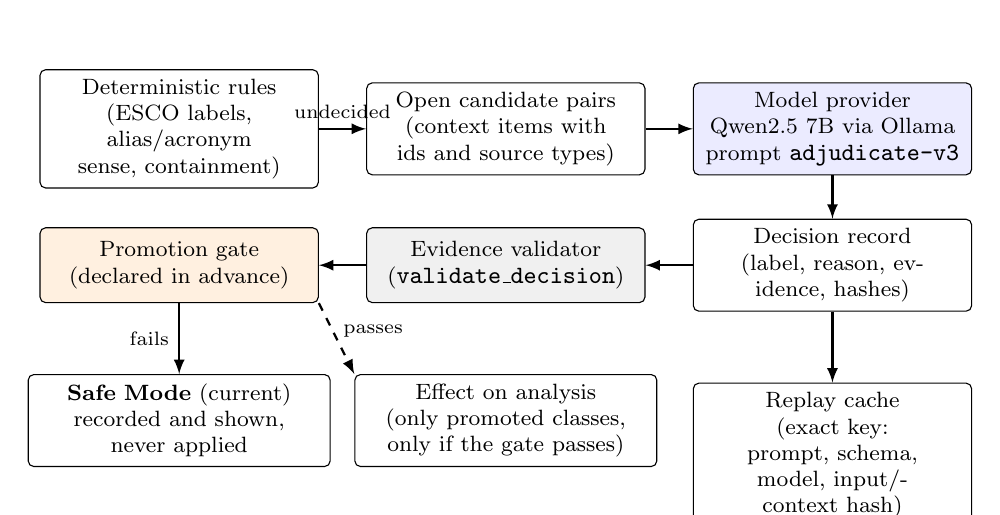
\begin{tikzpicture}[
  node distance=0.55cm and 0.6cm,
  box/.style={draw, rounded corners=2pt, align=center, font=\footnotesize, minimum height=0.95cm, text width=3.3cm, fill=white},
  rule/.style={box, fill=gray!12},
  model/.style={box, fill=blue!8},
  gate/.style={box, fill=orange!12},
  arr/.style={-{latex}, thick}]
\node[box] (rules) {Deterministic rules\\(ESCO labels, alias/acronym sense, containment)};
\node[box, right=of rules] (cand) {Open candidate pairs\\(context items with ids and source types)};
\node[model, right=of cand] (prov) {Model provider\\Qwen2.5 7B via Ollama\\prompt \code{adjudicate-v3}};
\node[box, below=of prov] (dec) {Decision record\\(label, reason, evidence, hashes)};
\node[rule, left=of dec] (val) {Evidence validator\\(\code{validate\_decision})};
\node[gate, left=of val] (gate) {Promotion gate\\(declared in advance)};
\node[box, below=0.9cm of gate, text width=3.6cm] (safe) {\textbf{Safe Mode} (current)\\recorded and shown,\\never applied};
\node[box, below=0.9cm of val, text width=3.6cm] (eff) {Effect on analysis\\(only promoted classes,\\only if the gate passes)};
\node[box, below=0.9cm of dec] (cache) {Replay cache\\(exact key: prompt, schema,\\model, input/context hash)};
\draw[arr] (rules) -- node[above, font=\scriptsize]{undecided} (cand);
\draw[arr] (cand) -- (prov);
\draw[arr] (prov) -- (dec);
\draw[arr] (dec) -- (val);
\draw[arr] (val) -- (gate);
\draw[arr] (gate) -- node[left, font=\scriptsize]{fails} (safe);
\draw[arr, dashed] (gate.south east) -- node[right, font=\scriptsize, pos=0.4]{passes} (eff.north west);
\draw[arr] (dec) -- (cache);
\end{tikzpicture}}
\caption[{Flow of a candidate pair through the semantic adjudication module}]{Flow of a candidate pair through the semantic adjudication module (from \code{docs/\allowbreak{}SEMANTIC\_INTELLIGENCE.md}, \code{semantic\_provider.py}, \code{semantic\_v3.py} and \code{engine\_config.json}). The dashed path has never been taken.}
\label{fig:architecture}
\end{figure}

\subsection{The validation workflow}

Figure~\ref{fig:workflow} shows the validation workflow. Its left branch, from the frozen benchmark through the blinded form, was carried out up to the reviewer responses. Its right branch, from independent labels through agreement, adjudication, frozen gold and gate evaluation, is implemented in \code{scripts/\allowbreak{}evaluation/\allowbreak{}semantic\_validation.py} but has not run, because no independent label set exists. The development scoring of this report is the middle path.

\begin{figure}[H]
\centering
\resizebox{\textwidth}{!}{%
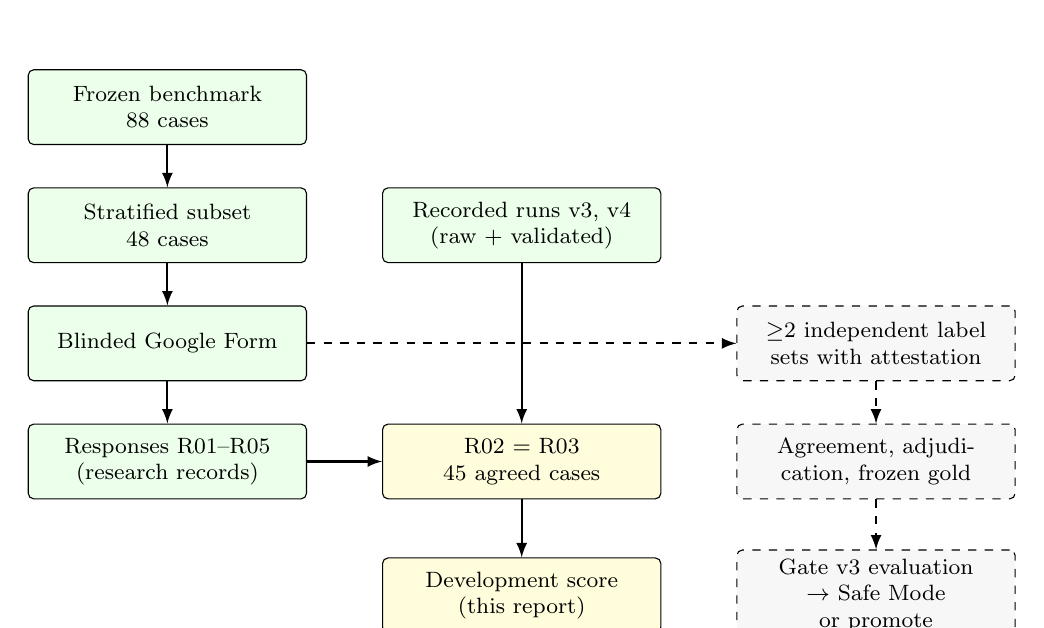
\begin{tikzpicture}[
  box/.style={draw, rounded corners=2pt, align=center, font=\footnotesize, minimum height=0.95cm, text width=3.3cm},
  done/.style={box, fill=green!8},
  dev/.style={box, fill=yellow!14},
  todo/.style={box, dashed, fill=gray!6},
  arr/.style={-{latex}, thick}]
% column 1: carried out
\node[done] (bench) at (0,0) {Frozen benchmark\\88 cases};
\node[done] (sub)   at (0,-1.5) {Stratified subset\\48 cases};
\node[done] (form)  at (0,-3.0) {Blinded Google Form};
\node[done] (resp)  at (0,-4.5) {Responses R01--R05\\(research records)};
% column 2: development scoring (this report)
\node[done] (runs)  at (4.5,-1.5) {Recorded runs v3, v4\\(raw + validated)};
\node[dev]  (agree) at (4.5,-4.5) {R02 = R03\\45 agreed cases};
\node[dev]  (score) at (4.5,-6.2) {Development score\\(this report)};
% column 3: not yet run
\node[todo] (ind)   at (9,-3.0) {$\geq$2 independent label sets with attestation};
\node[todo] (gold)  at (9,-4.5) {Agreement, adjudication, frozen gold};
\node[todo] (eval)  at (9,-6.2) {Gate v3 evaluation\\$\rightarrow$ Safe Mode or promote};
\draw[arr] (bench) -- (sub);
\draw[arr] (sub) -- (form);
\draw[arr] (form) -- (resp);
\draw[arr] (resp) -- (agree);
\draw[arr] (agree) -- (score);
\draw[arr] (runs) -- (agree);
\draw[arr, dashed] (form) -- (ind);
\draw[arr, dashed] (ind) -- (gold);
\draw[arr, dashed] (gold) -- (eval);
\end{tikzpicture}}
\caption[{The validation workflow}]{The validation workflow. Solid boxes: carried out. Shaded boxes: the development scoring reported here. Dashed boxes: implemented but not yet run (no independent labels); the gate evaluation will score the same recorded runs.}
\label{fig:workflow}
\end{figure}

\subsection{Integration with the rest of the project}

Model decisions never become source evidence. In Safe Mode they are stored next to the rule verdict and shown in the application's \emph{Semantic decisions} screens, but they change no demand, coverage, gap or recommendation. When the pipeline host cannot reach the model, recorded decisions are replayed only by an exact cache key: prompt version, schema, model, input hash and context hash. The replayed run's own gate result still applies. Reviewer responses are reachable through \code{/\allowbreak{}api/\allowbreak{}v1/\allowbreak{}semantic-validation/\allowbreak{}} endpoints and a \emph{Reviewer validation} screen. A development label is shown there only as a field marked \code{is\_human\_judgment: false} and never enters a metric.

\chapter{DESIGN SPECIFICATIONS}
\label{ch:design}

\section{Implementation Steps}
\label{sec:impl}

Table~\ref{tab:impl} lists the steps confirmed by the repository, in the order they were carried out, with their status. ``Implemented'' means the code and its outputs exist in the repository. ``Experiment'' means it was run and recorded but is not used in production. ``Proposed'' means it has not been built.

\begin{table}[p]
\centering
\footnotesize
\renewcommand{\arraystretch}{1.1}
\begin{tabularx}{\textwidth}{@{}p{0.4cm}X p{4.6cm} p{1.9cm}@{}}
\toprule
\textbf{\#} & \textbf{Step} & \textbf{Where (repository)} & \textbf{Status} \\
\midrule
1 & Build adjudication candidates from the pairs the rules leave open, and freeze them with hashes & \code{intelligence.py}, \code{scripts/\allowbreak{}semantic/\allowbreak{}freeze\_v3\_candidates.py} & Implemented \\
2 & Provider layer (Ollama, OpenAI-compatible, local transformers, deterministic fallback), decision schema v2, replay cache & \code{semantic\_provider.py} & Implemented \\
3 & Production prompt \code{adjudicate-v3} with label definitions and evidence items & \code{semantic\_v3.py} & Implemented \\
4 & Deterministic evidence validator & \code{semantic\_v3.validate\_decision} & Implemented \\
5 & Freeze the 88-case development benchmark; evaluate baseline, v2 and v3; apply the development gate & \code{evaluate\_v3.py}, \code{promotion\_gate.json} & Implemented (gate failed) \\
6 & Declare human-validation gates v2 (88 cases) and v3 (48-case subset) before any independent label & \code{semantic\_gate\_v2.json}, \code{semantic\_gate\_v3.json} & Implemented \\
7 & Build the validation package: stratified subset, blinded form generator, integrity check & \code{scripts/\allowbreak{}evaluation/\allowbreak{}semantic\_validation.py} & Implemented \\
8 & Independent-label import (requires an attestation), agreement, adjudication, gold freeze, gate evaluation & \code{semantic\_validation.py}, \code{semantic\_eval.py} & Implemented, not yet run \\
9 & Import reviewer responses as research records; compare; API and screen & \code{semantic\_responses.py}, \code{/\allowbreak{}api/\allowbreak{}v1/\allowbreak{}semantic-validation/\allowbreak{}} & Implemented \\
10 & Score recorded runs against reviewer responses (development and independent references) & \code{scripts/\allowbreak{}semantic/\allowbreak{}score\_against\_reviewers.py} & Implemented \\
11 & Prompt \code{adjudicate-v4} with the validator's rules and an ordered decision procedure & \code{semantic\_v3.build\_prompt\_v4} & Experiment, not adopted \\
12 & Independent human labels; refined decision rules; separate tuning and held-out sets; larger model & --- & Proposed \\
\bottomrule
\end{tabularx}
\caption[{Implementation steps and their status}]{Implementation steps and their status.}
\label{tab:impl}
\end{table}

\subsection{The evidence validator}

The validator, \code{validate\_decision}, is deterministic and is the main safety mechanism. For every model answer it checks the cited evidence against the inputs:
\begin{enumerate}
    \item each cited identifier must exist (otherwise \code{UNKNOWN\_REF}), and the quoted text must occur in that item (otherwise \code{QUOTE\_NOT\_IN\_ITEM});
    \item metadata items (taxonomy or normalisation facts) never count as evidence (\code{METADATA\_CITED});
    \item every definite relationship needs a cited item from the source side, i.e.\ the posting or syllabus (\code{NO\_SOURCE\_EVIDENCE});
    \item the meaning relations \SC, \PA, \CH, \RE{} and \PO{} also need a cited item from the concept side (\code{NO\_CONCEPT\_EVIDENCE});
    \item \PA{} and \CH{} need a direction justification and a cited directional item: an ESCO hierarchy or relation, or a course title, unit title or learning outcome (\code{NO\_DIRECTIONAL\_EVIDENCE});
    \item \SC{} on an alias or taxonomy-label case needs source text or a job title (\code{ALIAS\_SAME\_CONCEPT\_WITHOUT\_SOURCE\_TEXT}).
\end{enumerate}
Evidence that cannot be traced to the inputs leads to \code{REVIEW\_REQUIRED}, read downstream as \AM. Missing required evidence leads to \code{INSUFFICIENT\_EVIDENCE}, read as \IE. Only a decision that passes every rule is \code{MODEL\_SUPPORTED}. When the model itself answers \AM{} or \IE, the result is \code{MODEL\_SUGGESTED}, kept for review without effect.

\subsection{The v4 prompt experiment}

After the v3 results were compared with the reviewer responses, one prompt revision was tried. \code{adjudicate-v4} states the validator's evidence rules in the prompt and gives an ordered procedure: decide the sense; choose \SC{} only if the terms are interchangeable; a specific kind, product or provider is \CH; a broader area is \PA; shared meaning is \PO; association is \RE. Nothing else changed: the inputs, schema, validator, model and production configuration stayed the same. The project recorded the decision not to try further prompt variants against the same 45 cases, because each further attempt would be tuned on the same development answers.

\section{Tools and Technologies Used}
\label{sec:tools}

Only components verified in the repository, its configuration or its recorded runs are listed in Table~\ref{tab:tools}.

\begin{table}[H]
\centering
\small
\renewcommand{\arraystretch}{1.15}
\begin{tabularx}{\textwidth}{@{}p{3.4cm}X@{}}
\toprule
\textbf{Area} & \textbf{Technology (as verified)} \\
\midrule
Language and runtime & Python (3.14.7 on the run host, per \code{run\_meta.json}) \\
Language model & \code{qwen2.5:7b-instruct}, 7.6B parameters, Q4\_K\_M quantisation~\cite{qwen2024}; served by Ollama 0.34.4 on the project owner's Apple-silicon Mac; temperature 0 \\
Model interfaces & Ollama HTTP API; an OpenAI-compatible endpoint and a local \code{transformers} provider are configured but were unavailable in the recorded runs \\
Taxonomy & ESCO v1.2.1 (English classification and delta files); ESCO ontology with SKOS hierarchy~\cite{esco2024model} \\
Text processing & pdfplumber and poppler \code{pdftotext} (curriculum PDFs); scikit-learn TF-IDF (lexical similarity, concept clustering); pandas, NumPy; openpyxl (workbooks) \\
Back end and storage & FastAPI, Uvicorn, Pydantic; SQLAlchemy and Alembic over PostgreSQL; validation records kept as hash-identified JSON files \\
Front end & Flutter (Dart), including the \emph{Semantic decisions} and \emph{Reviewer validation} screens \\
Human validation & Google Forms (blinded form generated from the package); Excel export of responses \\
Testing & pytest (back end), \code{flutter test}; ruff (linting). The back-end suite reported 1{,}108 passed and 5 skipped on the project machine on 2026-10-22 \\
Report & \LaTeX{} with the CBIT template, biblatex, TikZ and pgfplots \\
\bottomrule
\end{tabularx}
\caption[{Tools and technologies verified in the project}]{Tools and technologies verified in the project.}
\label{tab:tools}
\end{table}

No embedding model or other neural model is part of the default configuration; the semantic backend is \code{tfidf}. No model weights were trained or fine-tuned.

\section{Results and Discussion}
\label{sec:results}

\subsection{Headline results on the development reference}

All figures in this section were recomputed for this report from the stored files by re-running the project's scoring code (\code{score\_against\_reviewers.py}) and an independent recalculation script, which agreed on every value. Table~\ref{tab:headline} gives the results on the 45 cases where R02 and R03 agree.

\begin{table}[H]
\centering
\small
\renewcommand{\arraystretch}{1.2}
\resizebox{\textwidth}{!}{%
\begin{tabular}{@{}lccccc@{}}
\toprule
\textbf{System} & \textbf{Correct} & \textbf{Accuracy} & \textbf{95\% CI} & \textbf{Commits} & \textbf{Right when committing} \\
\midrule
Fixed rules (baseline) & 0 / 45 & 0.00 & --- & 0 & --- \\
v3 raw & 15 / 45 & 0.33 & 0.21--0.48 & 44 & 15 / 44 (0.34) \\
v3 validated & 9 / 45 & 0.20 & 0.11--0.34 & 25 & 9 / 25 (0.36) \\
v4 raw & 12 / 45 & 0.27 & 0.16--0.41 & 45 & 12 / 45 (0.27) \\
v4 validated (as run) & 2 / 45 & 0.04 & 0.01--0.15 & 3 & 2 / 3 (0.67) \\
v4 validated, brackets removed$^{\dagger}$ & 9 / 45 & 0.20 & 0.11--0.34 & 26 & 9 / 26 (0.35) \\
\bottomrule
\end{tabular}}

\vspace{0.2cm}
{\footnotesize $^{\dagger}$Diagnostic only: the v4 model wrote cited identifiers as \code{[L1]}. Removing the brackets before validation shows what the prompt defect cost. The validator itself was not changed.}
\caption[{Results against the R02/R03 agreement (45 development cases)}]{Results against the R02/R03 agreement (45 cases, development reference, AI-assisted). Intervals are 95\% Wilson intervals.}
\label{tab:headline}
\end{table}

The provisional figures reported earlier in the project's discussions were checked against these results:
\begin{itemize}
    \item \textbf{R02 and R03 agree on 45 cases:} confirmed. They answered all 48 cases and disagree on 3 (bm1-043, bm1-045, bm1-046).
    \item \textbf{Model alone, 15/45:} confirmed.
    \item \textbf{Model with safety checks, 9/45:} confirmed.
    \item \textbf{Checked model, 9 of 25 answers:} confirmed. All 9 correct validated answers are commitments, since no abstention matched a reference.
    \item \textbf{Fixed rules, 0/45, ``always ambiguous'':} confirmed as 0/45. One detail differs. The fixed rules returned \AM{} for the 38 agreed cases on which they were run. The other 7 agreed cases are \code{DIAGNOSTIC} cases, for which the stored predictions contain no baseline output. On the whole benchmark, the baseline is \AM{} on all 75 non-diagnostic cases.
\end{itemize}

\subsection{The validator and abstention}

The validator withheld 20 of the 45 v3 answers (coverage 0.56, abstention rate 0.44). Of these, 14 were wrong raw answers and 6 were correct raw answers. It turned no wrong answer into a right one. It let through 25 answers, of which 9 were right and 16 wrong. Conditional accuracy therefore barely changed: 0.34 for raw answers, 0.36 for validated commitments. On this reference, the validator's main effect was to reduce the number of answers rather than to select the correct ones.

Table~\ref{tab:findings} shows which rules triggered. A case can trigger several rules. The most frequent finding was the absence of a cited concept-side item (17 cases). In 4 correct \SC{} answers (bm1-015, bm1-018, bm1-023, bm1-035), this was the only finding, so a correct answer was withheld only because the model did not cite the ESCO side. The v3 prompt asked for source-side evidence only and did not state this rule, which was the motivation for v4.

\begin{table}[H]
\centering
\small
\begin{tabular}{@{}lrr@{}}
\toprule
\textbf{Validator finding} & \textbf{v3 (cases)} & \textbf{v4 (occurrences)} \\
\midrule
\code{NO\_CONCEPT\_EVIDENCE} & 17 & 30 \\
\code{NO\_SOURCE\_EVIDENCE} & 7 & 41 \\
\code{ALIAS\_SAME\_CONCEPT\_WITHOUT\_SOURCE\_TEXT} & 5 & 4 \\
\code{METADATA\_CITED} & 4 & 0 \\
\code{QUOTE\_NOT\_IN\_ITEM} & 2 & 1 \\
\code{NON\_DEFINITE\_RELATIONSHIP} & 1 & 0 \\
\code{UNKNOWN\_REF} & 0 & 73 \\
\code{NO\_DIRECTIONAL\_EVIDENCE} & 0 & 7 \\
\bottomrule
\end{tabular}
\caption[{Validator findings on the 45 cases}]{Validator findings on the 45 cases. For v3 each finding is counted once per case. For v4 the project's scoring script counts occurrences (one case can cite several unknown identifiers).}
\label{tab:findings}
\end{table}

The v4 collapse to 2/45 has a mechanical cause. The prompt displays context items as \code{[L1]}, and v4 dropped v3's example \code{"ref": "<id>"}, so the model wrote the brackets into its citations. That produced 73 references to identifiers that do not exist. The validator correctly treated invented references as untraceable. With the brackets stripped for diagnosis only, v4 reaches the same 9/45 as v3.

\subsection{Why abstaining everywhere scores zero, and why that is not the whole story}

The fixed rules score 0/45 because exact-match accuracy counts an abstention as an error whenever the abstention label differs from the reference. Forty-two of the 45 references are definite relationships. The other three are \IE, and on those the baseline answered \AM, which is a different label. By construction, though, the baseline asserts no relationship at all: it makes no false \SC{} claim, no false hierarchy claim, and no claim without evidence. Its risk on committed answers is undefined, because it never commits. Its coverage is zero.

Exact-match accuracy therefore cannot rank these systems on its own. A system that commits often and is often wrong (v3 raw: 44 commitments, 29 wrong) can score higher than one that never commits, yet be more harmful downstream. The relevant view is the pair (coverage, conditional accuracy) together with the count of severe errors, which is exactly the view the gate takes~\cite{chow1970,geifman2017}. On this reference, the validated v3 system commits in 56\% of cases and is right in 36\% of its commitments. For comparison, the gate requires an overall accuracy of 0.80 and a precision of 0.90 for any class to be promoted.

\subsection{Strengths, weaknesses and safety mechanisms}

\paragraph{Strengths.} The model always produced schema-valid output (0 invalid outputs in 283 + 88 calls). Its answers were stable on repetition (20 of 20 identical relationships in both runs). Every decision is traceable through hashes to its exact inputs and prompt. The validator reliably caught evidence that did not exist in the inputs. The development gate, declared before the v3 outputs existed, failed on four of six checks (Table~\ref{tab:devgate}), and the system responded as designed by staying in Safe Mode.

\begin{table}[H]
\centering
\small
\begin{tabular}{@{}lrrc@{}}
\toprule
\textbf{Check (88-case benchmark, development labels)} & \textbf{Value} & \textbf{Threshold} & \textbf{Pass} \\
\midrule
Supported \SC{} alias predictions & 1 & $\geq 8$ & no \\
Precision of \SC{} on alias cases & 0.00 & $\geq 0.85$ & no \\
Lexical collisions supported as \SC & 2 & $0$ & no \\
Precision of \UN{} on alias cases & 0.846 & $\geq 0.85$ & no \\
Schema-valid rate & 1.00 & $\geq 0.98$ & yes \\
Metadata-only supported decisions & 0 & $0$ & yes \\
\bottomrule
\end{tabular}
\caption[{The development gate applied to the v3 run}]{The development gate applied to the v3 run (\code{qwen-270-v3/\allowbreak{}analysis/\allowbreak{}promotion\_gate.json}). The labels are the assistant's development labels, so this is a development check, not a validation.}
\label{tab:devgate}
\end{table}

\paragraph{Weaknesses.} The model did not recognise hierarchy. It never answered \PA{} or \CH{} on the 45 cases, although 16 references are hierarchical, and it over-used \SC{} (21 raw \SC{} answers against 10 \SC{} references). The validated system's 7 \SC{} commitments include 4 that the reviewers did not support. The v3 prompt did not tell the model the validator's evidence rules, so some correct answers were withheld for missing citations. The single prompt revision redistributed the errors instead of removing them (Chapter~\ref{ch:results}).

\paragraph{Safety mechanisms in place.} The mechanisms are:
\begin{itemize}
    \item the deterministic validator;
    \item pre-declared, versioned and hash-pinned gates;
    \item Safe Mode as the default outcome of any failure;
    \item replay only by exact cache key;
    \item strict separation of development labels, research records and independent labels;
    \item a mandatory attestation for independent labels.
\end{itemize}

The requirement for \emph{two independent reviewers} is encoded in the gate file (\code{min\_independent\_reviewers: 2}) and enforced by \code{apply\_gate}, which counts only label files marked \code{independent} and \code{model\_blind}. Such files can be created only through \code{import-form} or \code{import-sheet}, which refuse to run without a non-empty \code{--attestation}. The requirement that those reviewers \emph{did not use AI} is documented policy (\code{docs/\allowbreak{}INDEPENDENT\_REVIEWER\_BRIEF.md}). It is recorded through the attestation and enforced only to that extent: code can require the statement but cannot verify that it is true.

\chapter{PRESENTATION OF RESULTS}
\label{ch:results}

\section{Analysis of Findings}
\label{sec:analysisfindings}

All results in this chapter use the 45-case development reference described in Section~\ref{sec:analysis}. The tables are generated directly from the recomputed results file. They describe how the model behaves relative to two AI-assisted reviewers who agree with each other. They do not establish how accurate the model is.

\subsection{Overall picture}

Figure~\ref{fig:headline} summarises Table~\ref{tab:headline}. The validated v3 system and the bracket-corrected v4 system reach the same 9 of 45. The raw v4 answers are less accurate than the raw v3 answers, and on this sample the confidence intervals of all model variants overlap widely.

\begin{figure}[H]
\centering
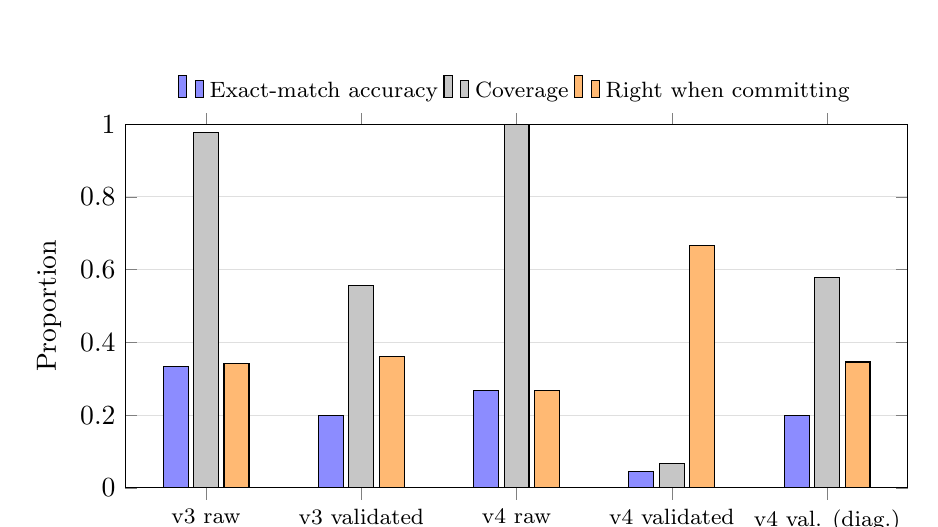
\begin{tikzpicture}
\begin{axis}[
    ybar, bar width=9pt, width=0.95\textwidth, height=6.2cm,
    ymin=0, ymax=1, ylabel={Proportion},
    symbolic x coords={v3 raw, v3 validated, v4 raw, v4 validated, v4 val. (diag.)},
    xtick=data, x tick label style={font=\footnotesize},
    legend style={at={(0.5,1.03)}, anchor=south, legend columns=3, font=\footnotesize, draw=none},
    ymajorgrids, grid style={gray!25},
    enlarge x limits=0.13]
\addplot[fill=blue!45] coordinates {(v3 raw,0.333) (v3 validated,0.2) (v4 raw,0.267) (v4 validated,0.044) (v4 val. (diag.),0.2)};
\addplot[fill=gray!45] coordinates {(v3 raw,0.978) (v3 validated,0.556) (v4 raw,1.0) (v4 validated,0.067) (v4 val. (diag.),0.578)};
\addplot[fill=orange!55] coordinates {(v3 raw,0.341) (v3 validated,0.36) (v4 raw,0.267) (v4 validated,0.667) (v4 val. (diag.),0.346)};
\legend{Exact-match accuracy, Coverage, Right when committing}
\end{axis}
\end{tikzpicture}
\caption[{Accuracy, coverage and conditional accuracy on the 45 development cases}]{Accuracy, coverage and conditional accuracy on the 45 development cases (values in Table~\ref{tab:headline}). ``v4 val.\ (diag.)'' is the diagnostic with citation brackets removed. The 0.67 of v4 validated rests on only 3 commitments.}
\label{fig:headline}
\end{figure}

\subsection{Confusion between equivalence, hierarchy, overlap and relatedness}

Table~\ref{tab:confraw} is the confusion matrix of the v3 raw answers. Three patterns stand out.

\begin{table}[H]
\centering
\small
\resizebox{\textwidth}{!}{\begin{tabular}{@{}lccccccccc@{}}
\toprule
\textbf{Reference} $\downarrow$ / \textbf{v3 raw} $\rightarrow$ & \rotatebox{70}{\SC} & \rotatebox{70}{\PA} & \rotatebox{70}{\CH} & \rotatebox{70}{\PO} & \rotatebox{70}{\RE} & \rotatebox{70}{\UN} & \rotatebox{70}{\AM} & \rotatebox{70}{\IE} & \textbf{Total} \\
\midrule
\SC & \cellcolor{green!25}\textbf{8} & \textcolor{gray!60}{0} & \textcolor{gray!60}{0} & \textcolor{gray!60}{0} & \textcolor{gray!60}{0} & \cellcolor{red!22}2 & \textcolor{gray!60}{0} & \textcolor{gray!60}{0} & 10 \\
\PA & \textcolor{gray!60}{0} & \textcolor{gray!60}{0} & \textcolor{gray!60}{0} & \textcolor{gray!60}{0} & \cellcolor{red!34}4 & \textcolor{gray!60}{0} & \textcolor{gray!60}{0} & \textcolor{gray!60}{0} & 4 \\
\CH & \cellcolor{red!50}7 & \textcolor{gray!60}{0} & \textcolor{gray!60}{0} & \cellcolor{red!16}1 & \cellcolor{red!28}3 & \cellcolor{red!16}1 & \textcolor{gray!60}{0} & \textcolor{gray!60}{0} & 12 \\
\PO & \cellcolor{red!40}5 & \textcolor{gray!60}{0} & \textcolor{gray!60}{0} & \textcolor{gray!60}{0} & \cellcolor{red!16}1 & \cellcolor{red!16}1 & \textcolor{gray!60}{0} & \textcolor{gray!60}{0} & 7 \\
\RE & \cellcolor{red!16}1 & \textcolor{gray!60}{0} & \textcolor{gray!60}{0} & \textcolor{gray!60}{0} & \cellcolor{green!25}\textbf{1} & \textcolor{gray!60}{0} & \textcolor{gray!60}{0} & \textcolor{gray!60}{0} & 2 \\
\UN & \textcolor{gray!60}{0} & \textcolor{gray!60}{0} & \textcolor{gray!60}{0} & \textcolor{gray!60}{0} & \textcolor{gray!60}{0} & \cellcolor{green!25}\textbf{6} & \textcolor{gray!60}{0} & \cellcolor{red!16}1 & 7 \\
\IE & \textcolor{gray!60}{0} & \textcolor{gray!60}{0} & \textcolor{gray!60}{0} & \textcolor{gray!60}{0} & \textcolor{gray!60}{0} & \cellcolor{red!28}3 & \textcolor{gray!60}{0} & \textcolor{gray!60}{0} & 3 \\
\midrule
\textbf{Predicted} & 21 & 0 & 0 & 1 & 9 & 13 & 0 & 1 & 45 \\
\bottomrule
\end{tabular}
}
\caption[{Confusion matrix, v3 raw answers (45 cases)}]{Confusion matrix, v3 raw answers against the R02/R03 agreement (45 cases). Diagonal in green, errors shaded by count.}
\label{tab:confraw}
\end{table}

\paragraph{Hierarchy is not recognised.} The \PA{} and \CH{} columns are empty: the model never asserted a hierarchical relation, although the reviewers gave one in 16 cases (12 \CH, 4 \PA). Narrower concepts were mostly called the same as their broader concept, and broader concepts were all called merely related.

\paragraph{\SC{} absorbs neighbouring classes.} Of the 21 raw \SC{} answers, 8 match the reference. The other 13 are 7 narrower concepts, 5 partial overlaps and 1 related pair. The model treats ``closely related'' as ``the same''.

\paragraph{Insufficient context is not recognised.} In the three cases where both reviewers judged that the context does not decide the relation, all short forms (``re'' twice, ``it''), the model answered \UN. That is a definite claim of a different sense rather than an admission that the text is insufficient.

Table~\ref{tab:errorcases} lists the three most frequent error categories, case by case. Because each case has exactly one reference and one raw answer, the categories do not overlap: together they account for 16 of the 30 raw errors. The remaining 14 errors are spread thinly: \CH~$\rightarrow$~\RE{} (3), \IE~$\rightarrow$~\UN{} (3), \SC~$\rightarrow$~\UN{} (2), and six single cases.

\begin{table}[H]
\centering
\small
\renewcommand{\arraystretch}{1.1}
\begin{tabularx}{\textwidth}{@{}p{1.5cm}X X@{}}
\toprule
\textbf{Case} & \textbf{Concept A (source)} & \textbf{Concept B (ESCO concept or topic)} \\
\midrule
\multicolumn{3}{@{}l}{\textbf{Narrower concept called same (\CH~$\rightarrow$~\SC): 7 cases}} \\
bm1-010 & MS Excel & use spreadsheets software \\
bm1-020 & MS Excel & use spreadsheets software \\
bm1-037 & cloud computing & cloud technologies \\
bm1-059 & google docs & office software \\
bm1-080 & Database Management Systems & database \\
bm1-084 & Convolutional Neural Network: The Convolution Operation & deep learning \\
bm1-086 & Python for Data Science & Python (computer programming) \\
\addlinespace
\multicolumn{3}{@{}l}{\textbf{Partial overlap called same (\PO~$\rightarrow$~\SC): 5 cases}} \\
bm1-002 & quality systems & quality control systems \\
bm1-031 & data privacy & data protection \\
bm1-052 & ict & computer technology \\
bm1-058 & conflict resolution & conflict management \\
bm1-060 & collaborate with colleagues & liaise with colleagues \\
\addlinespace
\multicolumn{3}{@{}l}{\textbf{Broader concept called related (\PA~$\rightarrow$~\RE): 4 cases}} \\
bm1-034 & financial planning & financial forecasting \\
bm1-053 & quality management & quality assurance procedures \\
bm1-063 & vector & vector line integrals \\
bm1-070 & Equations & equations solvable for y \\
\addlinespace
\bottomrule
\end{tabularx}

\caption[{The three most frequent error categories of the v3 raw answers}]{The three most frequent error categories of the v3 raw answers. The counts 7, 5 and 4 reproduce the figures reported during development.}
\label{tab:errorcases}
\end{table}

Two of the narrower-as-same cases appear twice under different case identifiers (``MS Excel'' in bm1-010 and bm1-020). The benchmark contains separate candidates for the same surface pair in different postings, so the 7 cases correspond to 6 distinct term pairs.

\subsection{Per-class behaviour}

Table~\ref{tab:prf} gives per-class precision, recall and F1. With 2 to 12 reference cases per class these values are very imprecise and are reported only to show the pattern. The pattern is consistent with the confusion matrix. \UN{} and \SC{} have the highest recall. \PA, \CH{} and \PO{} have zero recall. Validation lowers recall for \SC{} (0.80 to 0.30) without raising precision much (0.38 to 0.43), and moves 18 answers to \IE, none of which matches an \IE{} reference.

\begin{table}[H]
\centering
\small
\resizebox{\textwidth}{!}{\begin{tabular}{@{}lr|rrrr|rrrr@{}}
\toprule
 & & \multicolumn{4}{c|}{\textbf{v3 raw}} & \multicolumn{4}{c}{\textbf{v3 validated}} \\
\textbf{Class} & \textbf{Ref.} & \textbf{Pred.} & \textbf{P} & \textbf{R} & \textbf{F1} & \textbf{Pred.} & \textbf{P} & \textbf{R} & \textbf{F1} \\
\midrule
\SC & 10 & 21 & 0.38 & 0.80 & 0.52 & 7 & 0.43 & 0.30 & 0.35 \\
\PA & 4 & 0 & -- & 0.00 & -- & 0 & -- & 0.00 & -- \\
\CH & 12 & 0 & -- & 0.00 & -- & 0 & -- & 0.00 & -- \\
\PO & 7 & 1 & 0.00 & 0.00 & 0.00 & 1 & 0.00 & 0.00 & 0.00 \\
\RE & 2 & 9 & 0.11 & 0.50 & 0.18 & 5 & 0.20 & 0.50 & 0.29 \\
\UN & 7 & 13 & 0.46 & 0.86 & 0.60 & 12 & 0.42 & 0.71 & 0.53 \\
\AM & 0 & 0 & -- & -- & -- & 2 & 0.00 & -- & -- \\
\IE & 3 & 1 & 0.00 & 0.00 & 0.00 & 18 & 0.00 & 0.00 & 0.00 \\
\midrule
Macro-F1 (reference classes) & \multicolumn{5}{r|}{0.18} & \multicolumn{4}{r}{0.17} \\
\bottomrule
\end{tabular}
}
\caption[{Per-class precision, recall and F1, v3 raw and validated answers}]{Per-class precision (P), recall (R) and F1 for v3 raw and validated answers. ``--'': undefined because the class was never predicted, or never in the reference. Macro-F1 averages over the 7 classes present in the reference, counting undefined F1 as 0.}
\label{tab:prf}
\end{table}

For orientation only, and not as an evaluation (the gate applies to independent gold, which does not exist): among the validated system's 7 \SC{} commitments, 4 differ from the reviewers' answer (2 \PO, 1 \CH, 1 \RE). Gate v3 allows at most one false \SC.

\subsection{Effect of the v4 prompt}

Table~\ref{tab:confv4} shows the raw v4 answers. The ordered decision procedure reduced \SC{} answers from 21 to 6, and the model began to use \PA. But the errors moved instead of disappearing:
\begin{itemize}
    \item 6 narrower concepts were called \RE;
    \item 4 narrower concepts were called \PA, a reversal of direction. The narrower ``cloud computing'' was called broader than ``cloud technologies'' (bm1-037).
    \item 4 partial overlaps were called \RE.
\end{itemize}
Raw accuracy fell from 15 to 12. With the citation defect neutralised, the validated score equalled v3's 9. This is consistent with the project's conclusion that breadth and direction judgements are a limit of the 7B model rather than of the wording alone. The evidence for that conclusion is limited to one prompt revision, one model and 45 cases.

\begin{table}[H]
\centering
\small
\resizebox{\textwidth}{!}{\begin{tabular}{@{}lccccccccc@{}}
\toprule
\textbf{Reference} $\downarrow$ / \textbf{v4 raw} $\rightarrow$ & \rotatebox{70}{\SC} & \rotatebox{70}{\PA} & \rotatebox{70}{\CH} & \rotatebox{70}{\PO} & \rotatebox{70}{\RE} & \rotatebox{70}{\UN} & \rotatebox{70}{\AM} & \rotatebox{70}{\IE} & \textbf{Total} \\
\midrule
\SC & \cellcolor{green!25}\textbf{4} & \cellcolor{red!22}2 & \textcolor{gray!60}{0} & \textcolor{gray!60}{0} & \cellcolor{red!22}2 & \cellcolor{red!22}2 & \textcolor{gray!60}{0} & \textcolor{gray!60}{0} & 10 \\
\PA & \textcolor{gray!60}{0} & \textcolor{gray!60}{0} & \textcolor{gray!60}{0} & \cellcolor{red!22}2 & \cellcolor{red!22}2 & \textcolor{gray!60}{0} & \textcolor{gray!60}{0} & \textcolor{gray!60}{0} & 4 \\
\CH & \textcolor{gray!60}{0} & \cellcolor{red!34}4 & \textcolor{gray!60}{0} & \textcolor{gray!60}{0} & \cellcolor{red!46}6 & \cellcolor{red!22}2 & \textcolor{gray!60}{0} & \textcolor{gray!60}{0} & 12 \\
\PO & \cellcolor{red!16}1 & \cellcolor{red!16}1 & \textcolor{gray!60}{0} & \textcolor{gray!60}{0} & \cellcolor{red!34}4 & \cellcolor{red!16}1 & \textcolor{gray!60}{0} & \textcolor{gray!60}{0} & 7 \\
\RE & \cellcolor{red!16}1 & \textcolor{gray!60}{0} & \textcolor{gray!60}{0} & \textcolor{gray!60}{0} & \cellcolor{green!25}\textbf{1} & \textcolor{gray!60}{0} & \textcolor{gray!60}{0} & \textcolor{gray!60}{0} & 2 \\
\UN & \textcolor{gray!60}{0} & \textcolor{gray!60}{0} & \textcolor{gray!60}{0} & \textcolor{gray!60}{0} & \textcolor{gray!60}{0} & \cellcolor{green!25}\textbf{7} & \textcolor{gray!60}{0} & \textcolor{gray!60}{0} & 7 \\
\IE & \textcolor{gray!60}{0} & \textcolor{gray!60}{0} & \textcolor{gray!60}{0} & \textcolor{gray!60}{0} & \textcolor{gray!60}{0} & \cellcolor{red!28}3 & \textcolor{gray!60}{0} & \textcolor{gray!60}{0} & 3 \\
\midrule
\textbf{Predicted} & 6 & 7 & 0 & 2 & 15 & 15 & 0 & 0 & 45 \\
\bottomrule
\end{tabular}
}
\caption[{Confusion matrix, v4 raw answers (45 cases)}]{Confusion matrix, v4 raw answers (45 cases).}
\label{tab:confv4}
\end{table}

\subsection{Results by case kind}

Table~\ref{tab:bykind} breaks the results down by case kind. All six correct answers that validation withheld are alias cases (9 raw to 3 validated). Four of them were withheld only for a missing concept-side citation. The numbers per kind are too small for comparison between kinds.

\begin{table}[H]
\centering
\small
\begin{tabular}{@{}lrrrr@{}}
\toprule
\textbf{Case kind} & \textbf{Cases} & \textbf{v3 raw} & \textbf{v3 validated} & \textbf{v4 raw} \\
\midrule
\inputrows{generated/by_kind.tex}
\bottomrule
\end{tabular}
\caption[{Correct answers by case kind (45 development cases)}]{Correct answers by case kind (45 development cases).}
\label{tab:bykind}
\end{table}

\subsection{Reviewer agreement}

Table~\ref{tab:pairwise} gives Cohen's $\kappa$ and the number of agreements for every pair of the five reviewer records over the 48 cases. R02 and R03 agree far more closely ($\kappa=0.92$, 45 of 48) than any other pair ($\kappa$ between 0.56 and 0.76). This is consistent with their shared process of consulting an AI assistant first, but does not by itself establish it. The three R02/R03 disagreements concern ``Information Management'' versus ``knowledge management'' (\RE{} vs \PO) and the abbreviation ``ml'' in two cases, where R02 judged the context ambiguous.

\begin{table}[H]
\centering
\small
\begin{tabular}{@{}lccccc@{}}
\toprule
 & \textbf{R01} & \textbf{R02} & \textbf{R03} & \textbf{R04} & \textbf{R05} \\
\midrule
R01 & -- & 0.66 (34) & 0.64 (33) & 0.56 (30) & 0.59 (31) \\
R02 & 0.66 (34) & -- & 0.92 (45) & 0.63 (33) & 0.75 (38) \\
R03 & 0.64 (33) & 0.92 (45) & -- & 0.65 (34) & 0.73 (37) \\
R04 & 0.56 (30) & 0.63 (33) & 0.65 (34) & -- & 0.76 (38) \\
R05 & 0.59 (31) & 0.75 (38) & 0.73 (37) & 0.76 (38) & -- \\
\bottomrule
\end{tabular}

\caption[{Pairwise Cohen's $\kappa$ between the five reviewer records}]{Pairwise Cohen's $\kappa$ (number of agreements out of 48) between the five reviewer records. None of the records is an independent label set (Table~\ref{tab:reviewers}).}
\label{tab:pairwise}
\end{table}

The benchmark's development labels, written by an AI assistant, match the R02/R03 consensus in only 25 of the 45 cases. This supports the project's rule that development labels are for stratification and diagnostics only. It also shows that even two AI-informed sources can differ widely on these distinctions.

\subsection{Case-level record}

Table~\ref{tab:percase} lists every scored case so that each figure in this chapter can be traced. A bold label marks agreement with the reference.

{\small
\setlength{\tabcolsep}{4pt}
\begin{longtable}{@{}p{1.45cm}p{3.9cm}p{3.45cm}cccc@{}}
\caption[{All 45 development cases: reference and system answers}]{All 45 development cases: reference (R02 = R03) and system answers. SC = \SC, PA = \PA, CH = \CH, PO = \PO, RE = \RE, UN = \UN, AM = \AM, IE = \IE.}\label{tab:percase}\\
\toprule
\textbf{Case} & \textbf{Concept A} & \textbf{Concept B} & \textbf{Ref.} & \textbf{v3 raw} & \textbf{v3 val.} & \textbf{v4 raw} \\
\midrule
\endfirsthead
\toprule
\textbf{Case} & \textbf{Concept A} & \textbf{Concept B} & \textbf{Ref.} & \textbf{v3 raw} & \textbf{v3 val.} & \textbf{v4 raw} \\
\midrule
\endhead
\bottomrule
\endfoot
\inputrows{generated/per_case.tex}
\end{longtable}
}

\section{Comparison with Existing Work}
\label{sec:comparison}

No published study evaluates the same task on the same data, so a numerical comparison would be misleading. Table~\ref{tab:comparison} instead sets out how the related work differs from this project in task, data, method and metric. It identifies what each body of work contributes and what it does not settle for this project. No superiority is claimed in either direction.

\begin{table}[H]
\centering
\scriptsize
\renewcommand{\arraystretch}{1.25}
\begin{tabularx}{\textwidth}{@{}p{2.6cm}XXX@{}}
\toprule
\textbf{Work} & \textbf{Task and data} & \textbf{Method and metric} & \textbf{Difference from this project} \\
\midrule
STS pilot~\cite{agirre2012} & Graded similarity of sentence pairs & Human similarity scores; correlation with system scores & Scalar similarity, no relation type or direction; sentences, not terms with taxonomy context \\
Sentence-BERT~\cite{reimers2019} & Sentence embeddings for similarity search & Siamese fine-tuning; cosine similarity & Provides closeness, not the distinctions between \SC, \PA, \CH, \PO{} and \RE; the project uses TF-IDF and does not run an embedding model by default \\
Ontology matching~\cite{euzenat2013} & Correspondences between two ontologies & Typed correspondences (equivalence, subsumption, disjointness) & Closest in task; here one side is free text from postings and syllabi, with an explicit abstention option \\
Hierarchical classification~\cite{silla2011} & Assigning items to classes in a hierarchy & Hierarchy-aware evaluation & The project's labels are relation types, but its gate likewise treats direction errors as severe \\
Skill extraction and matching~\cite{sun2026,rosenberger2025,gonzalezgomez2025} & Skills in job text matched to ESCO; resume--job matching; taxonomy generation & Contrastive bi-encoders; shared embedding spaces; NER and relation extraction & Extraction and retrieval at scale; this project verifies a single typed relation for pairs the rules left open \\
LLM as judge~\cite{zheng2023} & Model judges compared with human preferences on chat answers & Agreement with human judgements; bias analysis & Same concern with model judgement reliability; here the model's labels gate data analysis and are kept advisory \\
LLM-assisted annotation~\cite{gilardi2023,veselovsky2023} & Annotation by models, and model use by crowd workers & Accuracy against expert labels; detection of model use & Explains why AI-assisted reviewer answers here are not treated as independent \\
Selective classification~\cite{chow1970,geifman2017} & Classifiers that may reject & Risk--coverage trade-off & The validator is a rule-based reject option; its thresholds are not learned, and coverage is reported alongside accuracy \\
\bottomrule
\end{tabularx}
\caption[{Comparison with related work by task, data, method and metric}]{Comparison with related work by task, data, method and metric.}
\label{tab:comparison}
\end{table}

Three differences matter most. First, this project evaluates a \emph{typed, directional} relation where much related work measures \emph{similarity}, so a high similarity score elsewhere says nothing about the hierarchy errors observed here. Second, the project scores what downstream would read after a deterministic validator, and reports abstention. Most published evaluations score raw outputs. Third, the project's reference is small and AI-assisted, while the cited studies rest on larger human-labelled datasets. Until independent labels exist, the project's figures cannot be placed on the same footing as published results.

\chapter{CONCLUSION}
\label{ch:conclusion}

\section{Summary of Findings}
\label{sec:summary}

This report evaluated the semantic relationship module of the Curriculum Intelligence project. The module asks a local language model to classify the relation between a term found in a posting or syllabus and an ESCO concept or curriculum topic, checks every answer with a deterministic evidence validator, and lets a pre-declared gate decide whether any answer may affect the analysis.

\begin{itemize}
    \item \textbf{Reference available.} Five reviewer records exist for the 48-case subset, but none is an independent label set. R02 and R03 consulted an AI assistant, and the process of the other three was not stated. The 45 cases on which R02 and R03 agree ($\kappa=0.92$) serve as a development reference only.
    \item \textbf{Verified results.} Every provisional figure was reproduced from the stored files:
    \begin{itemize}
        \item v3 raw: 15/45 (0.33);
        \item v3 validated: 9/45 (0.20), with 25 commitments of which 9 were right (0.36);
        \item fixed rules: 0/45. They abstained on every case they were run on; 7 diagnostic cases have no baseline output.
    \end{itemize}
    The 95\% intervals are wide (e.g.\ 0.11--0.34 for 9/45).
    \item \textbf{Main weakness.} The model does not separate equivalence from hierarchy, overlap and relatedness:
    \begin{itemize}
        \item it never answered \PA{} or \CH;
        \item it called narrower concepts the same (7 cases) and partial overlaps the same (5);
        \item it called broader concepts related (4);
        \item it answered \UN{} where the reviewers found the context insufficient (3).
    \end{itemize}
    \item \textbf{Safety checks.} The validator withheld 20 answers, 6 of them correct, and passed 25, of which 16 were wrong. It reliably rejects untraceable evidence, but on this reference it does not raise the proportion of correct commitments materially.
    \item \textbf{Prompt revision.} The v4 prompt reduced over-use of \SC{} but introduced direction reversals and more \RE{} answers, and it did not improve the validated score. It was not adopted.
    \item \textbf{Operating status.} The model remains in Safe Mode. The development gate failed for the v3 run, and gate v3 cannot be evaluated until two independent label sets exist. Model decisions are recorded and shown, never applied.
\end{itemize}

\section{Contributions to the Field}
\label{sec:contributions}

The contributions are practical and specific to this project. They do not establish general findings about language models.
\begin{enumerate}
    \item \textbf{An evidence-gated adjudication design.} A model's typed-relation decision reaches the analysis only after deterministic checks that its evidence exists in the inputs, covers both sides of the pair, and, for hierarchy, includes a structural directional fact. The design is implemented and tested.
    \item \textbf{A reproducible evaluation chain.} Frozen, hashed inputs; a stratified, blinded human-validation package; recorded model runs replayable by exact key; and scoring code that reports raw and validated answers, coverage and abstention with explicit denominators. Every number in this report was regenerated from these files.
    \item \textbf{A label-provenance discipline.} Development labels, AI-assisted research records and independent labels are stored apart and used for different purposes. Independent labels require an attestation, and AI-assisted answers can never count towards the gate.
    \item \textbf{A documented negative result.} The model's systematic failure on breadth and direction, and the failure of a targeted prompt revision to fix it, are recorded with case-level evidence, together with the decision not to keep tuning on the same development cases.
\end{enumerate}

\section{Future Work}
\label{sec:future}

The following stages are proposed. None of them has been carried out. They keep the existing label taxonomy and leave the gate unchanged.

\paragraph{Stage A --- Error diagnosis.} Classify every error with the existing labels. Separate breadth errors (\SC{} versus \CH/\PA/\PO) from association errors (\RE{} versus \PO) and sense errors (\UN). For each withheld answer, record which validator rule fired and whether the answer was right. Treat the three \IE{} references as a distinct question: when should the system say the text does not decide?

\paragraph{Stage B --- Rule and prompt refinement.} Make the hierarchy check explicit before \SC{} is allowed. For example, require the model to state whether either term names a kind, product, provider or part of the other, and to cite an ESCO hierarchy item or a course, unit or outcome when it claims a direction. Write explicit abstention criteria for short forms whose sense the context does not fix. Keep the validator at least as strict as now. Changes to the label taxonomy should be made only with a documented reason and a new schema version.

\paragraph{Stage C --- Development evaluation.} Tune only on designated development cases, such as cases of the 88-case benchmark that are \emph{not} in the 48-case subset, scored against their development labels as diagnostics. Record each change and its reason. Do not tune again on the 45 R02/R03 cases, which have already shaped v4.

\paragraph{Stage D --- Held-out evaluation.} Evaluate each revision once on cases not used to tune it. With 48 cases, a further split would leave too few cases per class to support conclusions, so a new frozen set drawn from the pipeline's candidates by the same stratified procedure is needed. Until then, any improvement should be described as a development observation, not as generalisation~\cite{cawley2010}.

\paragraph{Stage E --- Independent human validation.} Recruit at least two qualified reviewers who are not among R01--R05 and have not seen any model output or development label. Have them answer the existing blinded form without AI tools, following \code{docs/\allowbreak{}INDEPENDENT\_REVIEWER\_BRIEF.md}, and collect each reviewer's confirmation as the attestation. Then run the predefined procedure: agreement, adjudication by a named human, gold freeze, and evaluation against semantic-gate-v3 exactly as declared. If the gate fails, the model stays in Safe Mode. Any changed gate must be declared as a new version before the results it is applied to are seen.

\paragraph{Further experiments.} Run the same frozen candidates with a larger local model, to test whether breadth and direction errors are a limit of model size. Compare against a reference that uses ESCO's own hierarchy, where it exists, as a structural check on direction. Report coverage and conditional accuracy for every variant, not exact-match accuracy alone.




% Appendix and Code Attachments
\fontsize{10pt}{10pt}\selectfont

\begin{appendices}
\chapter{CODE ATTACHMENTS}
\label{app:code}

This appendix reproduces short excerpts of the project source that implement the parts of the module evaluated in this report. The lines are copied verbatim from the repository; the numbers in the margin are the line numbers in the original file. Excerpts are limited to the code discussed in the chapters, so the rest of each file is omitted.

\section{Relationship label schema}
\label{app:A1}
The eight labels and the definitions given to the model (Section~2.2, Table~2.1). The reviewer form uses the same eight labels. Source: \code{backend/\allowbreak{}app/\allowbreak{}knowledge\_engine/\allowbreak{}semantic\_provider.py}, lines 33--44.

\begin{lstlisting}[style=repo, firstnumber=33]
RELATIONSHIPS = ("SAME_CONCEPT", "PARENT", "CHILD", "RELATED", "PARTIAL_OVERLAP", "UNRELATED", "AMBIGUOUS",
                 "INSUFFICIENT_EVIDENCE")
RELATIONSHIP_DEFINITIONS = {
    "SAME_CONCEPT": "LEFT and RIGHT denote the same thing in this context",
    "PARENT": "LEFT is broader than RIGHT (RIGHT is a kind or part of LEFT)",
    "CHILD": "LEFT is narrower than RIGHT (LEFT is a kind or part of RIGHT)",
    "RELATED": "clearly associated, neither contains the other",
    "PARTIAL_OVERLAP": "they share part of their meaning",
    "UNRELATED": "different meanings (for example a different word sense)",
    "AMBIGUOUS": "the context supports more than one reading",
    "INSUFFICIENT_EVIDENCE": "the text does not allow a judgement",
}
\end{lstlisting}

\section{Ordered decision procedure of the v4 prompt experiment}
\label{app:A2}
The decision procedure added in prompt adjudicate-v4 (Section~4.1.2). It was evaluated and not adopted; production uses adjudicate-v3. Source: \code{backend/\allowbreak{}app/\allowbreak{}knowledge\_engine/\allowbreak{}semantic\_v3.py}, lines 203--213.

\begin{lstlisting}[style=repo, firstnumber=203]
DECISION_PROCEDURE_V4 = (
    "Decide in this order:\n"
    "1. Does LEFT, as used in the SOURCE CONTEXT, mean the RIGHT concept or something connected to it? If the source "
    "uses LEFT in another sense, answer UNRELATED. If the source does not let you tell, answer AMBIGUOUS (several "
    "readings fit) or INSUFFICIENT_EVIDENCE (nothing decides it).\n"
    "2. SAME_CONCEPT only if LEFT and RIGHT are interchangeable here: the same thing at the same breadth.\n"
    "3. CHILD if LEFT is one specific kind, instance, part, product, platform, vendor or tool of RIGHT. A named "
    "product or provider of a technology category is CHILD of that category, not SAME_CONCEPT.\n"
    "4. PARENT if LEFT is a broader area or category that includes RIGHT as one of its kinds or parts.\n"
    "5. PARTIAL_OVERLAP if they share part of their meaning but each also covers things the other does not.\n"
    "6. RELATED if they are associated (used together, a tool for, a prerequisite of) without sharing meaning.\n")
\end{lstlisting}

\section{Deterministic evidence validator}
\label{app:A3}
The rules every model answer must pass before it can reach the analysis (Section~4.1.1). Lines 31 to 279 of the file are omitted. Source: \code{backend/\allowbreak{}app/\allowbreak{}knowledge\_engine/\allowbreak{}semantic\_v3.py}, lines 28--30, 280--354.

\begin{lstlisting}[style=repo, firstnumber=28]
METADATA_TYPES = ("TAXONOMY_METADATA", "NORMALIZATION_METADATA")
DEFINITE = ("SAME_CONCEPT", "PARENT", "CHILD", "RELATED", "PARTIAL_OVERLAP", "UNRELATED")
MEANING_RELATIONS = ("SAME_CONCEPT", "PARENT", "CHILD", "RELATED", "PARTIAL_OVERLAP")
\end{lstlisting}

\noindent{\small\itshape Lines 31--279 omitted.}

\begin{lstlisting}[style=repo, firstnumber=280]
DIRECTIONAL_TYPES = ("ESCO_HIERARCHY", "ESCO_RELATION", "COURSE_TITLE", "UNIT_TITLE", "LEARNING_OUTCOME")


def validate_decision(out, c):
    """
    Deterministic gate over a model decision. Returns (final_state, findings).

    final_state:
      MODEL_SUPPORTED        definite relationship whose evidence passes every rule
      MODEL_SUGGESTED        AMBIGUOUS / INSUFFICIENT_EVIDENCE answered by the model (kept for review, no effect)
      REVIEW_REQUIRED        schema failure or evidence that cannot be traced to the inputs
      INSUFFICIENT_EVIDENCE  definite relationship without the required source evidence (downgraded)
    Rules: evidence present; each cited ref exists; the quote occurs in that item; the source type is OUR item's type
    (a model-claimed type that differs is recorded); metadata items never count; any definite relationship needs a
    SOURCE-side item; meaning relations (SAME/PARENT/CHILD/RELATED/PARTIAL) also need a CONCEPT-side item;
    PARENT/CHILD need a direction justification AND a cited directional item (DIRECTIONAL_TYPES); SAME_CONCEPT on alias/label candidates needs SOURCE_TEXT or JOB_TITLE.
    """
    findings = []
    schema = validate_output(out)
    if schema:
        return "REVIEW_REQUIRED", [f"SCHEMA: {e}" for e in schema]
    rel = out["relationship"]
    if rel not in DEFINITE:
        return "MODEL_SUGGESTED", ["NON_DEFINITE_RELATIONSHIP"]
    items = {it["id"]: ("LEFT", it) for it in c["left_items"]}
    items.update({it["id"]: ("RIGHT", it) for it in c["right_items"]})
    items.update({it["id"]: ("META", it) for it in c["metadata_items"]})
    valid = []
    for e in out.get("evidence", []):
        side_it = items.get(e["ref"])
        if side_it is None:
            findings.append(f"UNKNOWN_REF:{e['ref']}")
            continue
        side, it = side_it
        if len(_norm(e["quote"])) < 2:
            findings.append(f"EMPTY_QUOTE:{e['ref']}")
            continue
        if _norm(e["quote"]) not in _norm(it["text"]):
            findings.append(f"QUOTE_NOT_IN_ITEM:{e['ref']}")
            continue
        if e.get("source_type") and e.get("source_type") != it["source_type"]:
            findings.append(f"SOURCE_TYPE_MISLABELLED:{e['ref']}:{e.get('source_type')}->{it['source_type']}")
        if side == "META" or it["source_type"] in METADATA_TYPES:
            findings.append(f"METADATA_CITED:{e['ref']}")
            continue
        valid.append((side, it["source_type"]))
    untraceable = any(f.startswith(("UNKNOWN_REF", "QUOTE_NOT_IN_ITEM")) for f in findings)  # invented evidence
    has_left = any(s == "LEFT" for s, _ in valid)
    has_right = any(s == "RIGHT" for s, _ in valid)
    if not out.get("evidence"):
        findings.append("NO_EVIDENCE")
    if not has_left:
        findings.append("NO_SOURCE_EVIDENCE")
    if rel in MEANING_RELATIONS and not has_right:
        findings.append("NO_CONCEPT_EVIDENCE")
    if rel == "SAME_CONCEPT" and c["kind"] in ("ALIAS_SENSE", "AMBIGUOUS_TAXONOMY_LABEL") \
            and not any(s == "LEFT" and t in ("SOURCE_TEXT", "JOB_TITLE") for s, t in valid):
        findings.append("ALIAS_SAME_CONCEPT_WITHOUT_SOURCE_TEXT")
    if rel in ("PARENT", "CHILD") and not (out.get("direction_justification") or "").strip():
        findings.append("NO_DIRECTION_JUSTIFICATION")
    if rel in ("PARENT", "CHILD") and not any(t in DIRECTIONAL_TYPES for _, t in valid):
        # a shared word or one string inside another is never hierarchy: direction needs a structural fact
        findings.append("NO_DIRECTIONAL_EVIDENCE")
    blocking = {"NO_EVIDENCE", "NO_SOURCE_EVIDENCE", "NO_CONCEPT_EVIDENCE", "ALIAS_SAME_CONCEPT_WITHOUT_SOURCE_TEXT",
                "NO_DIRECTION_JUSTIFICATION", "NO_DIRECTIONAL_EVIDENCE"}
    if untraceable:
        return "REVIEW_REQUIRED", findings
    if any(f in blocking for f in findings):
        return "INSUFFICIENT_EVIDENCE", findings
    return "MODEL_SUPPORTED", findings


def effective_relationship(out, final_state):
    """What downstream may read: the model's relationship only when MODEL_SUPPORTED."""
    return out["relationship"] if final_state == "MODEL_SUPPORTED" else final_state
\end{lstlisting}

\section{Reading a model decision as downstream would}
\label{app:A4}
How a recorded decision becomes the validated answer that is scored in Chapters 4 and 5 (Section~3.2.2). Source: \code{scripts/\allowbreak{}semantic/\allowbreak{}score\_against\_reviewers.py}, lines 42--53.

\begin{lstlisting}[style=repo, firstnumber=42]
def validated(d, cand):
    """What downstream may read (same rule as scripts/semantic/evaluate_v3.py `effective`)."""
    if d is None:
        return None, ["NO_DECISION"]
    if d.get("decision_state") not in ("MODEL_SUGGESTED", "MODEL_SUPPORTED", "INSUFFICIENT_EVIDENCE", "REVIEW_REQUIRED"):
        return "AMBIGUOUS", [f"DECISION_STATE:{d.get('decision_state')}"]
    out = {k: d.get(k) for k in ("relationship", "reason", "evidence", "direction_justification", "alternatives",
                                 "uncertainty")}
    state, findings = v3.validate_decision(out, cand)
    if state in ("MODEL_SUPPORTED", "MODEL_SUGGESTED"):
        return d["relationship"], findings
    return ("INSUFFICIENT_EVIDENCE" if state == "INSUFFICIENT_EVIDENCE" else "AMBIGUOUS"), findings
\end{lstlisting}

\section{Cohen's kappa between two reviewers}
\label{app:A5}
The agreement statistic of Equation~3.4, used for Table~5.6. Source: \code{backend/\allowbreak{}app/\allowbreak{}knowledge\_engine/\allowbreak{}semantic\_eval.py}, lines 47--54.

\begin{lstlisting}[style=repo, firstnumber=47]
def cohen_kappa(a, b):
    n = len(a)
    if not n:
        return None
    po = sum(x == y for x, y in zip(a, b)) / n
    ca, cb = Counter(a), Counter(b)
    pe = sum(ca[k] * cb[k] for k in set(ca) | set(cb)) / (n * n)
    return None if pe == 1 else round((po - pe) / (1 - pe), 4)
\end{lstlisting}

\section{Applying the promotion gate}
\label{app:A6}
Every criterion of semantic-gate-v3 (Table~3.3) is checked; any failure leaves the system in SAFE\_MODE (Section~3.2.5). Source: \code{backend/\allowbreak{}app/\allowbreak{}knowledge\_engine/\allowbreak{}semantic\_eval.py}, lines 257--292.

\begin{lstlisting}[style=repo, firstnumber=257]
def apply_gate(gate, gold_rows, reviewers_agreement, system_result, label_sets):
    """Every check with its value and threshold; promotable classes only when the whole gate passes."""
    gold_cases = sum(1 for r in gold_rows if r["gold"])
    c = gate["criteria"]
    checks = {}

    def check(name, value, ok, threshold):
        checks[name] = {"value": value, "threshold": threshold, "pass": bool(ok)}
    check("independent_reviewers", len(label_sets), len(label_sets) >= c["min_independent_reviewers"], c["min_independent_reviewers"])
    check("gold_cases", gold_cases, gold_cases >= c["min_gold_cases"], c["min_gold_cases"])
    k = reviewers_agreement.get("kappa")
    if len(label_sets) >= 2:
        check("inter_rater_kappa", k, k is not None and k >= c["min_kappa_when_two_or_more_reviewers"],
              c["min_kappa_when_two_or_more_reviewers"])
    s = system_result
    check("accuracy", s["accuracy"], (s["accuracy"] or 0) >= c["min_accuracy"], c["min_accuracy"])
    check("macro_f1", s["macro_f1"], (s["macro_f1"] or 0) >= c["min_macro_f1"], c["min_macro_f1"])
    e = s["critical_errors"]
    check("false_same_concept", e.get("FALSE_SAME_CONCEPT", 0), e.get("FALSE_SAME_CONCEPT", 0) <= c["max_false_same_concept"], c["max_false_same_concept"])
    check("wrong_hierarchy_direction", e.get("WRONG_HIERARCHY_DIRECTION", 0),
          e.get("WRONG_HIERARCHY_DIRECTION", 0) <= c["max_wrong_hierarchy_direction"], c["max_wrong_hierarchy_direction"])
    fh = e.get("FALSE_PARENT", 0) + e.get("FALSE_CHILD", 0)
    check("false_parent_or_child", fh, fh <= c["max_false_parent_or_child"], c["max_false_parent_or_child"])
    check("unsupported_taxonomy_evidence", e.get("UNSUPPORTED_TAXONOMY_EVIDENCE", 0),
          e.get("UNSUPPORTED_TAXONOMY_EVIDENCE", 0) <= c["max_unsupported_taxonomy_evidence"], c["max_unsupported_taxonomy_evidence"])
    check("lexical_collision", e.get("LEXICAL_COLLISION", 0), e.get("LEXICAL_COLLISION", 0) <= c["max_lexical_collision"], c["max_lexical_collision"])
    passed = all(v["pass"] for v in checks.values())
    promotable = []
    if passed:
        for cls in gate["promotable_classes"]:
            pc = s["per_class"][cls]
            if pc["precision"] is not None and pc["predicted"] >= c["min_predictions_per_promoted_class"] \
                    and pc["precision"] >= c["min_precision_per_promoted_class"]:
                promotable.append(cls)
    return {"passed": passed, "checks": checks, "promotable_classes": promotable,
            "mode": "PROMOTE_VALIDATED_CLASSES" if passed and promotable else "SAFE_MODE"}
\end{lstlisting}

\section{Storing an independent label set only with an attestation}
\label{app:A7}
An independent label set cannot be created without a statement that the reviewer answered alone and without AI tools (Section~4.3.4). Source: \code{scripts/\allowbreak{}evaluation/\allowbreak{}semantic\_validation.py}, lines 709--731.

\begin{lstlisting}[style=repo, firstnumber=709]
def _store_labels(pkg, man, reviewer, rows, source_file, meta=None, attestation=None):
    """An INDEPENDENT_HUMAN_REVIEWER label set: it counts for agreement, gold and the gate, so it is stored only with
    a statement that the reviewer answered alone, from the case text, without AI tools and without seeing system
    output or another reviewer's answers (attestation: who confirmed it, and how). Responses that do not meet this go
    through import-responses instead."""
    try:
        name = se.check_reviewer(reviewer)
    except ValueError as exc:
        raise SystemExit(str(exc)) from exc
    if not (attestation or "").strip():
        raise SystemExit("an independent label set needs --attestation: who confirmed that the reviewer answered alone, "
                         "without AI tools, and how; otherwise import the responses with import-responses")
    out = pkg / "labels" / f"labels_{slug(name)}_v1.json"
    if out.exists():
        raise SystemExit(f"{out.name} exists; label sets are immutable")
    doc = {"benchmark": man["benchmark_version"], "benchmark_sha256": man["benchmark"]["sha256"], "package": man["package"],
           "reviewer": name, "reviewer_background": meta or {}, "label_version": "v1", "label_schema_version": man["label_schema_version"],
           "independent": True, "model_blind": True, "label_source": "INDEPENDENT_HUMAN_REVIEWER",
           "attestation": {"statement": attestation.strip(), "recorded_at": now()},
           "ingested_at": now(), "source_file_sha256": sha(Path(source_file).read_bytes()),
           "labels": rows, "labelled": sum(1 for r in rows if r["label"])}
    out.write_text(json.dumps(doc, indent=1, ensure_ascii=False))
    return out, doc
\end{lstlisting}


\end{appendices}

\fontsize{12pt}{12pt}\selectfont






% Change Bibliography to References
\renewcommand\bibname{REFERENCES}
\clearpage
\phantomsection
\addcontentsline{toc}{chapter}{REFERENCES}
\printbibliography


\end{document}